\documentclass[11pt,a4paper]{article}

\usepackage[utf8]{inputenc}
\usepackage{amsmath,amssymb,physics}
\usepackage{geometry}
\usepackage[bookmarks=false]{hyperref}  % recommended
\usepackage{tikz}
\usetikzlibrary{arrows.meta}
\usetikzlibrary{decorations.text}

\hypersetup{
  pdfencoding=unicode,
  psdextra,
  pdftitle={Resonance Quantum Theory (RQT), A Framework for Resonance-Base Structure and Interaction},
  pdfauthor={Olav Le Doigt}
}

\geometry{margin=2.4cm}

\newcommand{\paperversion}{v2}

\title{Resonance Quantum Theory (RQT):\\
A Framework for Resonance-Base Structure and Interaction\\
Conceptual Foundations and the Roton Quantum Model}

\author{Olav Le Doigt}
\date{\today\;\;(\paperversion)}

\begin{document}
\maketitle

% ABSTRACT pasted below

\begin{abstract}
The Resonance Quantum Theory (RQT) is a conceptual framework that interprets physical structure, interaction, and persistence as consequences of resonance organization rather than as properties imposed through fundamental particles, fields, or quantization rules. The framework begins from the assumption that localized resonance relationships can form within a continuous resonance-supporting continuum, giving rise to stable structures, interaction channels, and hierarchical organization across multiple scales.

In RQT, observable physical entities are viewed as dynamically maintained resonance structures. Stability arises through resonance closure, while interactions emerge through open and residual resonance channels connecting otherwise localized systems. Information, inertia, and binding are interpreted as consequences of the accommodation and reconfiguration of these resonance relationships. Matter and radiation are therefore treated not as fundamentally distinct categories, but as different manifestations of resonance organization within a common underlying framework.

The theory further proposes that physical structure develops hierarchically. Larger and more persistent systems emerge from networks of mutually stabilizing resonance configurations, while observable forces reflect residual effects of incomplete resonance closure. In this view, quantization, stability, and long-range interaction arise as natural consequences of resonance geometry and organization rather than as independent postulates.

To facilitate visualization, analysis, and numerical investigation, the Roton Quantum Model (RQM) is introduced as a discrete structural representation of the broader RQT framework. RQM projects resonance structures onto simplified resonance centers and channels, allowing complex resonance relationships to be described through a tractable geometric model while preserving the central concepts of closure, hierarchy, and interaction.

The purpose of this paper is to establish the conceptual foundations of RQT, define its principal structural concepts, introduce the relationship between RQT and RQM, and explore how resonance-based organization may provide a unified description of physical structure across scales.

\end{abstract}




% ==================================================== 1 INTRO =========================================================

\section{Introduction}

Nature exhibits persistent structure across an extraordinary range of scales. Atomic systems form stable molecules, molecules organize into complex materials, and larger structures emerge through increasingly intricate patterns of interaction. Despite their diversity, such systems share a common characteristic: they maintain coherence, stability, and recognizable identity while continuously interacting with their surroundings.

Modern physics provides highly successful mathematical descriptions of these phenomena. Quantum theory, quantum field theory, and relativity accurately predict a vast range of experimental observations and have established a remarkably consistent framework for understanding physical behavior. At the same time, many fundamental properties of physical systems are introduced through independent postulates, parameters, symmetries, or interaction rules. Stability, quantization, binding, charge, and long-range interaction are typically described within specialized theoretical frameworks, each optimized for a particular domain of observation.

This raises a broader conceptual question: might these apparently distinct phenomena arise from a common underlying organizational principle? Rather than beginning with particles, fields, or forces as fundamental entities, one may instead ask whether physical structure itself emerges from the formation and persistence of relationships between interacting systems.

The Resonance Quantum Theory (RQT) explores this possibility. The framework is based on the assumption that resonance relationships can form between localized structures and that these relationships may themselves become stable, persistent, and capable of further interaction. In this view, physical systems are understood not primarily as isolated objects but as dynamically maintained networks of resonance relationships. Stability, interaction, and hierarchy are interpreted as consequences of the organization of these relationships across different scales.

The purpose of RQT is not to replace successful physical descriptions, but to investigate whether a common resonance-based framework can provide a deeper conceptual basis from which a wide range of observed phenomena may emerge. The theory therefore focuses on the formation of resonance structures, the development of stable interaction channels, and the mechanisms through which increasingly complex systems can arise from comparatively simple assumptions.

To facilitate visualization and quantitative exploration of these concepts, a simplified structural representation referred to as the Roton Quantum Model (RQM) is introduced later in this work. RQM provides a discrete geometric description of resonance structures and their interactions while remaining rooted in the broader conceptual framework established by RQT.

The following chapters develop the fundamental concepts of the theory, introduce the notion of resonance channels and closure, and examine how physical structure may emerge from the organization of resonance relationships across multiple levels of complexity.

% ————————————————————

%\section{Motivation}

%Conceptual challenges in modern physics.

%\subsection{Matter and Interaction}
%\subsection{Quantization}
%\subsection{Inertia and Stability}
%\subsection{Emergence and Hierarchy}



% ==================================================== 2 FOUNDATION =========================================================

\section{Conceptual Foundations}

The conceptual foundation of RQT is intentionally minimal. Rather than beginning with particles, fields, or forces, it starts from the possibility that stable identities may emerge through persistent relationships. Once such an identity has formed, it may itself participate in further relationships, allowing increasingly complex structures to arise through repeated application of the same principle. Figure 1 summarizes this recursive concept, which is developed throughout the remainder of this section.

\begin{figure}[!ht]
\centering

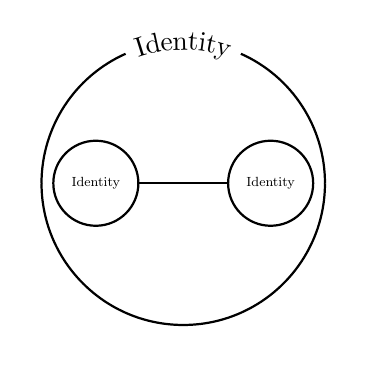
\begin{tikzpicture}[ scale=0.6, transform shape, >=Stealth, every node/.style={font=\small}, line width=0.8pt]
\def\R{3.0}
\def\r{0.90}
\def\d{1.85}
%\draw (0,0) circle (\R);
\def\Gap{24}
\draw (180:\R) arc (180:{90+\Gap}:\R);
\draw ({90-\Gap}:\R) arc ({90-\Gap}:0:\R);
\draw (180:\R) arc (180:360:\R);
\path[decorate, decoration={text along path, text={Identity}, text align=center, raise=-3pt}] (315:\R) arc (315:-135:\R);
\draw (-\d,0) circle (\r);
\draw ( \d,0) circle (\r);
\node[font=\footnotesize] at (-\d,0) {Identity};
\node[font=\footnotesize] at ( \d,0) {Identity};
\draw (-\d+\r,0) -- (\d-\r,0);
\end{tikzpicture}

\caption{Recursive Formation of Identity}
\label{fig:rqt_identity}
\end{figure}

The remainder of this section develops the individual conceptual elements of this recursive process.

\subsection{Persistence and Self-Resonance}

\emph{Before a structure can interact, it must first persist.}

The Resonance Quantum Theory begins with a minimal conceptual assumption: the existence of a continuum capable of supporting oscillatory behavior. The framework does not initially specify the origin, composition, or geometry of this continuum. It merely assumes that localized oscillatory configurations may arise within it.

An oscillatory configuration does not necessarily constitute a persistent structure. Of particular interest are configurations that repeatedly return to compatible states. Such recurrence allows an oscillation to maintain its identity over extended durations and establishes the possibility of persistence.

Within RQT, persistence is regarded as the first prerequisite for the emergence of structure. A persistent oscillatory configuration forms a self-maintaining cycle whose future evolution remains compatible with its preceding states. This process is referred to as self-resonance. At the conceptual level adopted here, self-resonance may be regarded as the simplest form of persistent resonance behavior.

The precise nature of such self-resonant configurations is not specified at this stage. Their significance lies not in their detailed structure, but in the fact that they provide a mechanism through which stable and persistent patterns may arise. Once persistence is established, increasingly complex forms of coupling, interaction, and organization become possible.

RQT therefore considers persistent self-resonant configurations as the conceptual starting point from which higher-order resonance structures can emerge.


\subsection{Stability and Identity}

\emph{Persistence allows oscillatory behavior to remain. Stability allows it to become structure.}

A persistent oscillatory configuration does not necessarily remain unchanged. Local adjustments, interactions, and ongoing accommodation may continuously influence its evolution. Within RQT, stability therefore does not imply rigidity or immutability. Instead, a structure is considered stable when it repeatedly returns to sufficiently compatible states, allowing its characteristic behavior to persist despite ongoing change.

Such stable resonance structures represent the first distinguishable configurations within the framework. Their identity does not arise from a fixed internal composition, but from the persistence of recognizable resonance properties over time. A stable structure may therefore be characterized through its phase relationships, recurrence behavior, and interaction potential rather than through a permanently defined geometry.

The continued existence of a stable resonance structure also preserves information about its formation and evolution. This information is not regarded as a separately stored quantity, but as an intrinsic consequence of the ongoing resonance process itself. The present state of a structure remains connected to preceding states through a continuous resonance flow, allowing distinctions and relationships to persist over time.

Once stable resonance structures emerge, they may participate in increasingly complex forms of coupling and organization. Stability therefore provides the foundation upon which interaction, relationship formation, and higher-order resonance structures can develop.

Within RQT, stable resonance structures constitute the first identifiable building blocks from which larger resonance networks and hierarchical organizations may arise.


\subsection{Interaction and Relationship Formation}

\emph{Interaction creates relationships. Relationships create shared identity.}

Stable resonance structures do not exist in complete isolation. Whenever the state of one structure influences the evolution of another, an interaction is established. The precise mechanism through which this influence occurs is not specified at this stage. It is sufficient to recognize that persistent structures may affect one another and thereby participate in a common process of development.

Within RQT, interactions are significant not merely because they modify existing structures, but because they give rise to relationships. A relationship represents an organized connection between two or more structures whose future evolution can no longer be described entirely independently. Through interaction, participating structures begin to share aspects of their resonance behavior and thereby become part of a larger organizational whole.

The emergence of a relationship introduces an additional level of identity. While the participating structures may remain individually distinguishable, the relationship itself acquires significance as a persistent element of the overall resonance organization. From a higher-level perspective, the relationship may therefore be regarded as a structure in its own right.

Relationships need not possess equal strength or persistence. Some may remain weak and contribute only limited influence on the participating structures. Others may develop increasingly shared resonance organization, causing their behavior to become progressively interdependent. The distinction between weak, strong, and highly persistent relationships is therefore not regarded as fundamental, but as a consequence of the degree to which resonance organization becomes shared.

As relationships persist, they may themselves participate in further interactions and form new relationships with other structures. In this manner, interaction becomes a mechanism through which increasingly complex organizations can emerge. Relationship formation therefore provides the foundation for higher-order resonance structures and the hierarchical organization discussed in the following section.


\subsection{Emergence and Hierarchical Organization}

\emph{Every stable organization becomes a candidate for higher-order organization.}

The formation of a relationship does not necessarily result in a new persistent identity. Many relationships may remain transient, while others persist only for limited durations. Within RQT, higher-order structures emerge when relationships acquire sufficient stability to participate in the resonance organization of their surroundings as identifiable entities in their own right.

The persistence of a relationship depends on the degree of compatibility between the participating structures. Compatibility is not regarded as a binary property, but as a condition that may develop through continued interaction. As structures influence one another, adjustments in their relative states may increase or decrease the stability of the relationship. Persistent relationships therefore arise not merely from interaction itself, but from the ability of interacting structures to accommodate one another sufficiently to maintain a shared organization over time.

When a relationship becomes persistent, a new level of identity emerges. This higher-order identity is not simply the sum of its constituents. Instead, it may exhibit resonance capabilities, interaction possibilities, and organizational properties that were not available to the participating structures independently. The emergence of such capabilities constitutes the basis of higher-order structure formation within the framework.

The formation of a new identity may also alter the accessibility of previously available relationships. Certain interactions may become enhanced, while others may become reduced, concealed, or effectively internalized within the newly formed structure. Emergence therefore introduces not only new possibilities for interaction, but also new forms of organization and selective accessibility.

Once established, higher-order identities may themselves participate in further relationship formation. The same principles that govern the emergence of lower-level structures may therefore operate recursively across multiple levels of organization. In this manner, increasingly complex resonance structures can arise without requiring additional foundational assumptions.

RQT consequently interprets hierarchy not as a separate organizing principle, but as a natural consequence of persistent relationship formation, emergent identity, and the continual development of new resonance capabilities across successive levels of organization.


\subsection{Accessible and Enclosed Structure}

\emph{Stability favors enclosure. Enclosure creates selective accessibility.}

The emergence of higher-order structures introduces an important distinction between the internal organization of a structure and the properties it exposes to its surroundings. Within RQT, stable structures are not assumed to make all aspects of their internal resonance organization equally accessible. Instead, the formation of persistent identities naturally leads to varying degrees of accessibility between internal and external levels of organization.

This tendency arises from the continuous search for stable resonance configurations. As relationships become organized into higher-order structures, the participating components may reduce their dependence on external interactions by establishing increasingly stable internal relationships. The resulting organization can allow parts of the internal structure to become less directly involved in the structure's interactions with its surroundings.

Enclosure is therefore not regarded as a separate organizing principle, but as a natural consequence of stability. A structure that reduces unnecessary external dependencies may become less susceptible to disturbance and thereby maintain its identity more effectively over time. The degree of enclosure achieved by a structure depends on both its internal organization and the conditions imposed by its environment.

The emergence of enclosure creates selective accessibility. Some properties of a structure remain available for further relationship formation and interaction, while others become partially or fully internalized within the structure itself. As a result, the externally accessible behavior of a structure need not reveal the full complexity of its internal organization.

The accessible properties of a structure define how it participates in higher-order organization. Internal relationships, however, may continue to influence the behavior and stability of the structure even when they are not directly accessible from the outside. In this sense, every emergent structure may possess both an externally visible identity and an internal organization that extends beyond what is immediately available to its surroundings.

RQT therefore regards accessibility and enclosure as complementary aspects of stable organization. The formation of higher-order structures not only creates new identities and interaction possibilities, but also establishes boundaries between what remains externally available and what becomes incorporated into the internal organization of the structure.



\subsection{Framework Assumptions and Scope}

\emph{Complexity is not introduced. Complexity is accumulated.}

The preceding sections have established the conceptual foundations upon which the Resonance Quantum Theory is developed. Rather than beginning with particles, forces, fields, or predefined physical laws, the framework starts from a small set of organizational assumptions and explores the consequences that follow from them.

RQT assumes the existence of a continuum capable of supporting oscillatory behavior. Within this continuum, persistent oscillatory configurations may arise and maintain their identity through self-resonance. Persistent structures may influence one another, form relationships, and develop increasingly stable forms of organization. Relationships that become sufficiently persistent may themselves emerge as higher-order identities capable of participating in further relationship formation.

The framework does not assume that all configurations persist. Persistence is itself regarded as a non-trivial property. Only structures that remain sufficiently stable can continue to participate in subsequent organization and relationship formation. Increasing levels of complexity may therefore arise through the continued accumulation of persistent relationships across multiple levels of organization.

From these assumptions emerge the concepts of identity, interaction, hierarchy, accessibility, and enclosure. Higher-order structures are understood not as independent organizing principles, but as consequences of recursive relationship formation and the development of persistent resonance organization.

At this stage, the framework intentionally refrains from specifying the detailed mechanisms through which such structures are realized. It does not initially assume particles, forces, charge, mass, spacetime geometry, probabilistic state descriptions, or specific interaction laws. These concepts, if required, are expected to emerge as effective descriptions of deeper resonance processes rather than as fundamental starting points.

The purpose of the framework is therefore not to introduce additional elementary entities, but to investigate how increasingly complex physical organization may arise from a minimal set of resonance-based assumptions. The following sections explore how specific resonance structures, interaction mechanisms, and observable physical phenomena may emerge from these principles.



%Oscillatory Capability
 %       ↓
%Persistence
 %       ↓
%Identity → Relationships → Emergence → Hierarchy → Enclosure → Selective Accessibility → Higher-Order Identity
 %                ↑_____________________________________________________________________________|


\begin{figure}[t]
\centering

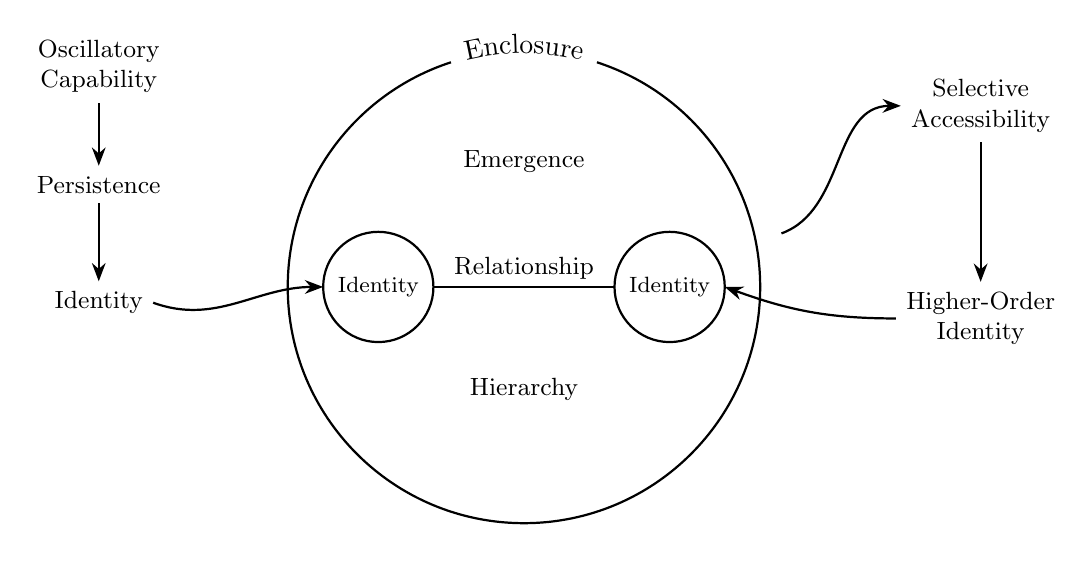
\begin{tikzpicture}[
    >=Stealth,
    every node/.style={font=\small},
    line width=0.8pt
]

\def\R{3.0}
\def\r{0.70}
\def\d{1.85}
	
%\draw (0,0) circle (\R);
\def\Gap{18}
% Upper left
\draw (180:\R)
      arc (180:{90+\Gap}:\R);
% Upper right
\draw ({90-\Gap}:\R)
      arc ({90-\Gap}:0:\R);
% Lower half
\draw (180:\R)
      arc (180:360:\R);
      
    
%\node[ fill=white, inner xsep=4pt, inner ysep=1pt ] at (90:\R) {Enclosure};

\path[
    decorate,
    decoration={
        text along path,
        text={Enclosure},
        text align=center,
        raise=-1pt
   }
]
(315:\R) arc (315:-135:\R);

\draw (-\d,0) circle (\r);
\draw ( \d,0) circle (\r);

\node[font=\footnotesize] at (-\d,0) {Identity};
\node[font=\footnotesize] at ( \d,0) {Identity};

\draw (-\d+\r,0) -- (\d-\r,0);
\node[above] at (0,-0.03) {Relationship};

\node at (0,1.60) {Emergence};
\node at (0,-1.30) {Hierarchy};

\node[align=center] (osc) at (-5.4, 2.8){Oscillatory\\Capability};
\node (per) at (-5.4,1.3){Persistence};
\node (id) at (-5.4,-0.2){Identity};

\draw[->] (osc) -- (per);
\draw[->] (per) -- (id);
\draw[->](id.east) to[out=-20,in=180] (-\d-\r,0);

\node[align=center] (acc) at (5.8,2.3){Selective\\Accessibility};
\node[align=center] (hid) at (5.8,-0.4){Higher-Order\\Identity};

\draw[->](3.27,0.68) to[out=20,in=180] (acc.west);
\draw[->](acc)--(hid);
\draw[->](hid.west) to[out=180,in=-20] (\d+\r,0);

\end{tikzpicture}

\caption{Conceptual foundations of the Resonance Quantum Theory}
\label{fig:rqt_foundations}
\end{figure}





% --------------------------
\iffalse
Future Chapter:
Resonance Continuum and Spacetime
--> Space-time is continuum of perfectly closed resonance channels. Disturbences will open a resonance channel - a Sonon or rather a Sonon-Pair.

Future Chapter:
- Prime-Periods: Will they be more stable?
- Do we have and indications in nature that prime numbers are favoured or avoided for some parts?

Vibrations -> Oscillations -> Self-Resonance ...

TODO:
Prime periods, factorization hierarchy, resonance richness of composite periods versus prime periods, possible implications for stability and resonance accessibility.

Distance is not necessarily separation in space, but separation and compatibility in identity.
\fi
% ————————————————————





% ==================================================== 2 THEORY =========================================================


\section{The Resonance Quantum Theory}

\emph{Conceptual foundations of the framework.} 
\vspace{0.6em} 

\noindent
The conceptual foundations introduced the recursive emergence of persistent identities without assuming a specific physical realization. The Resonance Quantum Theory extends this framework by describing how such identities interact, organize, and evolve through resonance itself. The concepts introduced in this section remain independent of any particular geometric or discrete representation and therefore form the theoretical basis upon which the Roton Quantum Model is later constructed.

\subsection{Resonance as a Fundamental Principle}
Resonance is not treated in RQT as a special physical phenomenon occurring only under particular conditions. Instead, it is adopted as the fundamental principle by which oscillatory structures establish, maintain, and evolve stable organization.

The conceptual foundations introduced the emergence of persistent identities through recursive relationship formation without assuming a particular physical realization. The next step is to identify the principle that determines whether such relationships remain transient or develop into stable structures. RQT proposes that this principle is resonance.

In its most general sense, resonance describes the mutual adaptation of oscillatory systems whenever their evolving states become sufficiently compatible. Such adaptation may involve phase, characteristic frequencies, spatial organization, or other structural properties, without requiring any specific geometric representation. While many interactions remain temporary, resonance provides the possibility for oscillatory systems to organize into persistent configurations.

From the perspective of RQT, resonance is therefore not regarded as a consequence of existing physical objects. Rather, stable physical objects are understood as consequences of persistent resonance. Resonance is treated as the organizing principle from which increasingly stable structures may emerge, interact, and recursively form higher-order identities.

The following sections develop this framework by introducing the continuum in which resonance occurs, the formation of localized resonance structures, and the mechanisms by which resonance accommodates, stabilizes, and eventually gives rise to observable physical systems.


\subsection{The Resonance Continuum}

\emph{RQT does not begin by asking what space is made of. It begins by asking what is minimally required for stable resonance to exist.}
\vspace{0.6em} 

\noindent
RQT does not attempt to explain the origin or fundamental nature of the substrate in which resonance occurs. Instead, it adopts the minimal assumption that a continuum exists which is capable of supporting persistent oscillatory organization. Beyond this requirement, no particular physical interpretation is assumed.

From the perspective of RQT, this continuum should not initially be identified with physical space or spacetime. Rather, it represents the possibility for oscillatory structures to emerge, persist, and mutually influence one another. Observable notions such as separation, spatial distance, and temporal evolution are not taken as fundamental prerequisites but are considered possible emergent descriptions of stable resonance organization.

This represents a conceptual inversion of the usual viewpoint. Rather than assuming that resonance occurs within a pre-existing spacetime, RQT explores the possibility that the observable notions of space and time arise from the formation, separation, and continued interaction of persistent resonance identities. The theory therefore begins with distinction and relationship rather than with metric geometry.

Only one assumption is required: sufficiently compatible oscillatory structures may establish persistent relationships. These relationships provide the basis from which increasingly organized resonance structures may emerge and subsequently interact through newly available resonance pathways. The concepts of distance, propagation, and geometry are introduced only insofar as they become meaningful descriptions of these emerging relationships.

A consequence of this viewpoint is that the underlying mechanism giving rise to the first persistent oscillatory capability need not itself remain directly accessible. If higher-order resonance structures arise through successive stages of resonance organization, then the deeper levels from which these structures originate may become intrinsically concealed by the same principles of resonance confinement that later govern stable physical systems. In this sense, the apparent simplicity of a persistent oscillation may itself be the observable residue of a deeper resonance organization whose internal structure no longer participates directly in accessible interactions.

The following sections therefore take the existence of this resonance continuum as a conceptual starting point and investigate how localized resonance structures emerge, interact, accommodate one another, and eventually give rise to stable physical organization.

\subsection{Distinct Resonance Structures}

\emph{The first observable property of a resonance structure is not its location, but its persistent distinction.}
\vspace{0.6em} 

The existence of a resonance continuum alone does not imply the existence of distinguishable structures. Many oscillatory configurations may remain transient, continuously emerging and dissolving without establishing persistent organization. RQT therefore distinguishes between arbitrary oscillation and oscillatory organization that becomes sufficiently persistent to form a distinct resonance structure.

A distinct resonance structure is not initially defined by position, geometry, dimensionality, or physical extent. Instead, it is defined by the continued persistence of its oscillatory organization and by its distinguishability from the surrounding resonance continuum. Distinction therefore precedes localization. Only after stable relationships emerge may geometric descriptions become meaningful.

Persistent distinction also implies continuity. A resonance structure possesses both a history and the potential for continued evolution, not because information is explicitly stored, but because its oscillatory organization remains continuously connected to its own past. The present state is therefore understood as the ongoing evolution of the same resonance process rather than as a sequence of independently recreated states.

From the perspective of RQT, a resonance structure remains part of the observable resonance organization only insofar as this continuity persists. A structure that became completely disconnected from all continuing resonance relationships would cease to participate in the same observable organization. Whether such complete decoupling is possible remains an open question. Everyday physical structures, however, exhibit persistent relationships over extended periods, suggesting that stable resonance organization generally preserves continuity rather than abandoning it.

RQT begins not with localized objects, but with persistent distinction. Identity emerges from the continued existence of a persistent resonance organization. Interaction, separation, and geometry emerge only thereafter through the relationships established between such structures.

Distinct resonance structures therefore provide the first entities capable of participating in persistent interaction. The following section examines how these structures influence one another, adapt through resonance, and establish the relationships from which increasingly organized physical systems emerge.

\subsection{Resonance Interaction}

\emph{Interaction begins whenever the continued evolution of one distinct resonance structure influences that of another.}
\vspace{0.6em} 

The existence of distinct resonance structures inevitably allows the possibility of interaction. Whenever two structures participate in one another’s continued evolution, they no longer develop independently. Their oscillatory organization begins to adjust through mutual influence, giving rise to resonance interaction.

Interaction should not be understood as a discrete event but as a continuous process. Some interactions remain transient, producing only temporary adjustments before the participating structures continue independently. Others persist, allowing the interacting structures to accommodate one another over extended periods. Resonance interaction therefore represents a dynamic process whose consequences depend on the continued compatibility of the participating structures rather than on the mere occurrence of a single encounter.

Accommodation does not necessarily imply observable change. Highly compatible resonance structures may remain in continuous interaction while exhibiting little or no apparent evolution because their oscillatory organization is already mutually consistent. Interaction therefore exists whenever resonance structures contribute to one another’s continued organization, regardless of whether this contribution manifests as rapid adaptation or as stable equilibrium.

The degree to which an interaction contributes to the continued organization of the participating structures determines its significance within the evolving resonance system. Persistent interactions gradually become part of the resonance organization itself, while transient interactions leave little lasting influence. The following sections investigate how such persistent interactions organize into stable resonance relationships and eventually give rise to the structured resonance pathways that characterize stable physical systems.

% -----------

\subsection{Resonance Accommodation}

\emph{Interaction becomes organization when resonance structures begin to accommodate one another.}
\vspace{0.6em} 

Resonance interaction is not a fixed relation between otherwise unchanged structures. Continued interaction influences the evolution of all participating resonance structures and may gradually alter the compatibility of their oscillatory organization. RQT refers to this process as resonance accommodation.

Accommodation is understood as a continuous and mutual process. The participating structures do not merely act upon one another from the outside; their evolving resonance organization becomes increasingly interdependent. This may involve adjustments in phase, characteristic periods, relative organization, or other resonance properties, without requiring any particular geometric representation at this stage.

Successful accommodation allows interacting structures to develop a partially shared resonance evolution. Their future states can no longer be described independently, because each structure contributes to the continued organization of the other. Where compatibility increases, the interaction may persist and become part of a larger resonance organization. Where compatibility cannot be maintained, the interaction may remain transient, weaken, or lead to reorganization.

Accommodation does not necessarily produce visible change. Two highly compatible structures may remain in continuous interaction while exhibiting little apparent evolution, precisely because their resonance organization is already mutually consistent. Stable resonance therefore represents not the absence of interaction, but a condition in which further accommodation is only minimally required.

In realistic systems, accommodation is not limited to isolated pairs. Every resonance structure may participate in several simultaneous interactions, each contributing to its continued evolution. Resonance accommodation therefore occurs within a network of mutually constraining relationships, where the persistence of any one interaction depends on its compatibility with the wider resonance organization.

RQT does not require that resonance structures consciously or globally optimize their organization. It proposes only that interactions capable of maintaining compatible shared evolution remain available for continued organization, while incompatible interactions tend to remain transient or reorganize. In this sense, accommodation does not create resonance; it reveals which resonance relationships can persist.

The persistence of accommodated interaction provides the conceptual basis for the structured resonance relationships introduced in the following sections.

% --------------------------
\iffalse
Fin: So something had to be, which made the universe build such long distances (between galaxies and stars) these are the stable structures, this does minimize resonance inconsistency. So when we can not do it while being close to each other, we need distance. So too much closeness of matter seams to inverse or repell the process, as soon as the innermost sonons can not accomodate or "flee" anymore then the system explodes again leading into momentum - and the need for time to accomadate into resonant systems again.)
\fi
% --------------------------

\subsection{Stability and Persistence}

\emph{Stability denotes the persistence of an organized resonance process, not the absence of change.}
\vspace{0.6em} 

A resonance organization becomes stable when its continued evolution preserves the distinction and internal coherence by which it can be identified. Such stability does not require every oscillatory state or resonance relationship to remain unchanged. Rather, the organization must retain sufficient continuity for its present evolution to remain connected to its preceding states.

Even a simple resonance relationship contains both internal and external aspects. Internally, the participating structures sustain the mutual organization through which they form a distinguishable system. Externally, each participating structure may remain exposed to additional resonance influences arising from its surrounding environment or from relationships at another level of organization. Stability therefore depends not only on internal compatibility, but also on the capacity of the system to accommodate changing external demands.

External or internal changes may introduce resonance mismatch into an existing organization. A stable system can respond by adjusting and redistributing this mismatch across its participating relationships while preserving the organization as a whole. The resulting changes may occur within subordinate structures, within the relationships that hold them together, or in the system’s external relations, without necessarily interrupting its persistent identity.

Stability is therefore dynamic rather than static. A stable resonance organization may undergo continuous internal adjustment while remaining distinguishishable as the same continuing process. The more effectively such adjustments remain bounded within the existing organization, the less they disturb its higher-level identity.

Persistence and stability describe related but distinct aspects of this continuation. Persistence refers to the continued existence of a distinguishable resonance organization. Stability refers to its capacity to preserve that continued identity under changing resonance conditions.

When an imposed resonance mismatch can no longer be accommodated within the existing organization, the system may reorganize, separate, or dissolve into configurations capable of more persistent resonance evolution. Separation is therefore not necessarily the failure of accommodation, but may itself restore compatibility among the remaining resonance structures.

A stable resonance system is thus not isolated from change. Its stability lies in maintaining a recognizable organization while continuously accommodating the resonance influences in which it participates.


\subsection{Resonance Distribution Across Hierarchies}

\emph{Resonance organization is sustained not only by local accommodation, but by the distribution of accommodation demands across nested structures and relationships.}
\vspace{0.6em} 

A distinguishable resonance structure may itself contain subordinate resonance structures, while simultaneously participating in larger resonance organizations. RQT therefore considers physical organization to be hierarchical: an identity may act as a coherent whole at one level while remaining internally composed of interacting sub-identities at another.

Changes introduced at one level need not remain confined to that level. An external resonance influence may alter a relationship within the larger identity, while the resulting mismatch is redistributed through its internal organization. Conversely, changes arising within a subordinate structure may propagate outward and affect the relationships through which the higher-level identity is maintained.

The response of a resonance system therefore depends on the distribution of its available accommodation capacity. Some disturbances may be absorbed locally, requiring only minor adjustment within a limited part of the structure. Others may be distributed across several internal relationships, producing a broader but still coherent reorganization. Where the existing organization cannot accommodate the imposed mismatch, the disturbance may extend to the system boundary and alter its external relationships.

This distribution is not assumed to follow a predetermined geometric pathway. It reflects the evolving compatibility of the resonance relationships participating in the system. Accommodation proceeds through those parts of the organization capable of contributing to a more persistent shared evolution, while strongly incompatible relationships may weaken, reorganize, or separate.

A higher-level identity may therefore remain stable even while its internal resonance organization changes substantially. Its persistence depends not on the immutability of its components, but on whether the combined adjustments preserve the relationships through which the whole remains distinguishable. In this sense, stability at one level may be supported by continuous reorganization at another.

Resonance structures are also constrained by their wider environment. Because each identity participates in several simultaneous relationships, no accommodation occurs in isolation. A configuration compatible with one relationship may introduce mismatch into another. Persistent organization therefore emerges from the distributed accommodation of multiple, mutually constraining resonance influences.

Where accommodation succeeds, previously distinct structures may participate in a more coherent higher-level identity. Where it fails, the existing organization may release subordinate structures, alter its external relationships, or separate into new resonance systems. Formation and dissolution are thus complementary outcomes of the same underlying process: the redistribution of resonance toward configurations capable of continued organization.

This hierarchical view prepares the transition from general resonance processes to the structured relationships through which persistent resonance organization can be represented. The following sections introduce the resonance channels, closures, and enclosures that describe these enduring forms of shared resonance evolution.





% ==================================================== 2 RESONANCE CHANNELS AND CLOSURE =========================================================

\section{Resonance Channels and Closure}

\emph{The formation of observable structure.}
\vspace{0.6em} 

The preceding sections described resonance organization as a continuing process of interaction, accommodation, redistribution, and persistence. As the number of participating structures and relationships increases, however, a purely process-based description becomes increasingly difficult to follow. A compact representation is therefore required for the persistent organization produced by these processes.

RQT introduces the concepts of resonance channels and resonance closure for this purpose. These concepts do not add new physical ingredients to the theory. A resonance channel represents the continuing organization of a persistent interaction, while closure describes the extent to which that interaction has become incorporated into a self-consistent resonance structure.

A channel is therefore not assumed to be a material conduit or a geometrically defined path. At the general level of RQT, it expresses a persistent resonance relationship whose organization contributes to the identities of the participating structures and, where applicable, to the higher-level identity they form together.

Not every resonance relationship becomes fully closed. Some remain partially accommodated, externally exposed, or distributed across wider resonance systems. The distinction between open, residual, and closed resonance organization will later allow increasingly complex systems to be described without requiring their complete internal evolution to be followed at every level.

These concepts remain independent of any particular microscopic geometry. The Roton Quantum Model will later propose specific structural representations of resonance channels, nodes, closures, and enclosures. At this stage, channels and closure are introduced only as the general relational language through which persistent resonance organization can be described.


\subsection{Resonance Channels}

\emph{A resonance channel is the persistent organization of a distinguishable resonance interaction.}
\vspace{0.6em} 

Resonance interaction may be transient, diffuse, distributed, or continuously changing. Where such interaction becomes sufficiently persistent and organized to contribute to the continuing identity of a resonance structure or system, RQT represents it as a resonance channel.

A channel is therefore not an additional physical substance, conduit, or pre-existing path through space. It is the relational organization through which resonance structures participate in a shared evolution. The interaction is fundamental; the channel is its persistent and distinguishable form.

A resonance channel need not initially possess a defined geometric length, width, curvature, or orientation. At the general level of RQT, it is characterized by the persistence, compatibility, and organization of the interaction it represents. Specific geometric properties may arise only when the channel is embedded within a more detailed structural model.

Channels may differ in the way they participate in a resonance system. Some form persistent relationships between identifiable counterparts. Others remain externally exposed, distributed across several interactions, or only partially organized around a dominant partner. A channel may therefore be open, relationally occupied, redirected, or incorporated into a more completely closed resonance organization.

The existence of a channel also does not require an unchanging interaction partner. What persists may be the organized mode of coupling itself, while the structures contributing to it change over time. This allows a channel to represent both stable pairwise relationships and persistent interactions with a distributed resonance environment.

A realized channel contributes to the identities of the structures it connects. Where several resonance structures become organized through persistent channels, their relationships may together establish a distinguishable higher-level resonance identity. Channels therefore do not merely connect pre-existing objects; they participate in defining what those objects and larger systems become.

The number and mutual compatibility of channels available to a given identity are not determined by general RQT alone. They depend on the adaptability and internal organization of the resonance structure supporting them. The Roton Quantum Model later represents these constraints through specific channel types, channel counts, and structural arrangements.


\subsection{Open and Closed Channels}

A realized resonance channel may remain open or become increasingly closed according to how fully its interaction is incorporated into the resonance organization under consideration.

An open resonance channel forms a persistent relationship between distinguishable resonance structures, but remains at least partly available to further accommodation. Its organization may still respond substantially to external resonance influences, shift between competing relationships, or participate in the formation of a larger resonance system. Openness therefore does not imply that the channel is weak or temporary. It indicates that the relationship has not yet become fully internalized within a stable resonance organization.

A closed resonance channel is a persistent interaction that has become predominantly incorporated into the internal organization of a resonance system. Closure does not terminate or deactivate the relationship. Rather, the participating structures sustain one another through an increasingly self-consistent resonance process, making the channel part of the identity of the resulting system.

The distinction between open and closed channels is not necessarily binary. Continued accommodation may gradually increase closure, while changing resonance conditions may partially or temporarily reopen a previously closed channel. During such reopening, the system becomes more accessible to external accommodation and may redistribute, redirect, or reorganize the relationship.

Whether a channel is considered open or closed also depends on the identity level being examined. A channel may be closed within one resonance system while the resulting higher-level identity remains open to additional relationships of its own. Closure at one level therefore does not imply isolation from the wider resonance environment.

By becoming closed, a channel changes more than its own relational state. Its incorporation alters the resonance organization of the participating structures and thereby changes which further relationships remain compatible and available to the resulting identity.

Closure changes the future compatibility landscape of the resulting identity.


\subsection{Residual Resonance}

\emph{Residual resonance is resonance influence that remains externally accessible without being fully organized into a closed relationship.}
\vspace{0.6em} 

Residual resonance may arise where a realized channel is only incompletely closed, temporarily reopened, or continuously affected by redistribution within its enclosing structure. In such cases, part of the interaction remains accessible to the wider resonance environment even though the principal relationship is sustained internally.

Residual resonance may also arise from an available channel mode that has not become organized around a distinct counterpart. Its influence then remains distributed across the surrounding resonance environment rather than forming a directed, partner-specific channel. Another compatible structure may respond to this distributed influence and, through continued accommodation, establish a realized resonance channel.

Residual resonance therefore differs from a closed channel both in organization and relational specificity. A closed channel sustains a distinguishable relationship within an enclosure, whereas residual resonance may remain diffuse, externally exposed, and shared among several possible interactions.

The strength and distribution of residual resonance may later be related to the emerging separation and geometry of resonance structures. Their quantitative representation, including possible distance-dependent laws, belongs to the more specific development of the Roton Quantum Model.

\subsection{Resonance Closure}

\emph{Resonance closure occurs when a persistent interaction becomes sufficiently accommodated to form an internally sustaining part of a resonance identity.}
\vspace{0.6em}

A realized resonance channel may remain externally exposed, compete with alternative relationships, or require continued adjustment. Through accommodation, however, it may become increasingly self-consistent and internalized within a larger resonance organization.

Closure does not terminate the interaction. It changes its relational role: an externally negotiable relationship becomes an internally supporting component of the resulting system. This transition may be gradual, and changing resonance conditions may partially reopen or reorganize a previously closed channel.

Closure also changes which further relationships remain compatible. As a channel becomes internalized, equivalent external coupling modes may be reduced, redirected, or removed. Depending on the identity, this may saturate a channel type or leave other compatible channels available.

Closure does not imply perfect isolation. Residual influence and weak environmental redistribution may remain. It denotes a state in which the relationship is predominantly sustained within the internal organization of the resonance system, thereby preparing the emergence of a higher-level identity.

\subsection{Resonance Stabilization}

\emph{Closure favours stability by converting externally negotiable resonance relationships into internally sustaining organization.}
\vspace{0.6em}

Reduced external coupling may arise through several distinct processes. A relationship may become internally closed through resonance locking, while rapid rotation or other continuing variation may prevent a stable counterpart from forming and leave only residual external influence.

Alternatively, interacting sub-identities may reorganize into a new combined resonance mode in which the original channel becomes unavailable and different internal or external channels emerge.

Closure, dynamical decoupling, and internal mode reorganization may therefore all stabilize a resonance system, but through different changes in its underlying organization.

\subsection{Channel Availability and Saturation}

\emph{A resonance identity can realize only those channels that remain compatible with its existing resonance organization.}
\vspace{0.6em}

Channel availability describes the forms of persistent interaction that an identity is capable of sustaining. An available channel mode is not yet a realized relationship; it becomes one only when compatible structures establish a sufficiently persistent interaction.

Realizing or closing a channel changes the organization of the identity and may preserve, reduce, redirect, or remove the compatibility required for additional channels. Several channels can coexist only where their accommodation demands remain mutually compatible.

An identity is saturated with respect to a channel type when no additional compatible channel of that type can be realized within its present organization. Residual interaction may nevertheless remain, and reopening, weakening, or reorganization of existing channels may later restore availability.

The number and arrangement of channels supported by particular physical identities are not determined by general RQT, but by the more specific structures proposed within the Roton Quantum Model.

\textbf{Channel availability may be reduced by realized or closed relationships; where no further compatible channel of a given type remains, the identity is saturated with respect to that channel type.}


\subsection{Resonance Enclosure}


\emph{A resonance enclosure is a persistent higher-level identity sustained by relationships that have become predominantly internal to its organization.}

When resonance channels close, the participating structures do not lose their subordinate identities. Their resonance possibilities are instead constrained and reorganized by the combined system. The resulting enclosure can persist and interact as a distinguishable identity of its own.

An enclosure is not necessarily a spatial shell or an isolated system. Its boundary is defined by the distinction between relationships that sustain the identity internally and those through which it remains connected to the wider resonance environment.

Formation of an enclosure does not end accommodation. Continued internal redistribution may allow the system to enter more coherent resonance states and establish internal modes that were unavailable to its constituents separately. In doing so, previously external channel availability may be reduced or reorganized, while new relationships become possible within the enclosure.

Different enclosures may internalize different channel types or different combinations of relationships. Their stability therefore depends not only on the degree of closure, but also on whether the resulting internal organization can continue to accommodate external resonance demands.

An enclosure may itself retain open channels, residual resonance, and further channel availability. It can therefore participate as a sub-identity in a larger enclosure, extending resonance organization across successive hierarchical levels.

%\emph{Resonance closure occurs when a persistent interaction becomes sufficiently accommodated to form an internally sustaining part of a resonance identity.}
%\vspace{0.6em} 

%\subsection{Resonance Locking}

%\emph{Resonance locking is the self-reinforcing process through which a realized interaction converges toward closure.}
%\vspace{0.6em} 

As accommodation progresses, one shared resonance organization may become increasingly dominant over competing configurations. Further adjustments then reinforce the same relationship, dynamically confining the interaction to an increasingly compatible mode.

Locking may require substantial reorganization within the participating identities. Existing channels may shift or temporarily reopen, while resonance that cannot be incorporated into the emerging closure may be redistributed or released.

The process need not be instantaneous or irreversible. Locking may remain incomplete, become temporarily stable, or reverse under changing resonance conditions. Where it succeeds, the realized channel becomes increasingly internalized and may culminate in channel closure and the formation or reorganization of a resonance enclosure.

Locked and closed are therefore not fully synonymous. Closure describes how completely a relationship has become incorporated into the internal organization of an enclosure. Locking describes the dynamical capture of that relationship and its resistance to leaving the established resonance mode. A channel may consequently be strongly closed yet comparatively easy to reopen, or strongly locked while closure remains incomplete.

Closure describes the resulting relational structure; locking describes its dynamical capture and retention.


% ==================================================== 3 RELATIONAL SEPARATION =========================================================

%Relational Separation and Emergent Geometry
%    Relational Position
%    Resonance Distance
%    Phase and Propagation
%    Distance Locking
%    Emergent Dimensionality

\section{Relational Separation and Emergent Geometry}

The preceding sections described how persistent resonance relationships may close and become internal to a higher-level resonance enclosure. Closure, however, is not the only way in which several resonance identities can form a stable organization.

Distinct identities may remain individually recognizable while participating in a shared resonance structure at the same organizational level. Additional identities may join this structure without necessarily becoming subordinate components of a recursively enclosed identity. Their relationships instead form a lateral resonance network whose stability depends on the mutual compatibility of the complete arrangement.

Such networks introduce relational separation. The participating identities must remain sufficiently distinct to preserve their individual organization, yet sufficiently compatible to sustain persistent resonance relationships. Separation is therefore not initially understood as distance within a pre-existing metric space. It describes the relational distinction required for several identities to coexist within a common resonance organization.

\subsection{Relational Position}

A resonance identity acquires a relational position through the pattern of interactions in which it participates. Its position is initially defined not by coordinates, but by its relationships to neighbouring identities and by the role it occupies within the wider resonance organization.

Two otherwise equivalent identities may therefore occupy different relational positions because they participate in different channel configurations. As these configurations become persistent and repeatable, they establish an ordered distinction between the identities involved.

Relational position provides the first basis for later concepts such as neighbourhood, direction, and location. These concepts do not precede resonance organization, but arise from persistent differences within it.

\subsection{Resonance Separation}

Resonance separation describes the relational distinction maintained between identities that participate in a shared organization. It expresses the degree and form of differentiation required for their individual resonance structures to remain distinguishable while continuing to interact.

This separation need not initially be metric or uniquely defined. The same pair of identities may be closely related through one channel type while remaining more weakly connected through another. A geometric notion of distance becomes meaningful only where resonance relationships establish repeatable and mutually comparable separations.

Separation may also contribute to stability. Greater proximity does not necessarily improve accommodation. Where nearby resonance structures impose mutually incompatible demands, a larger separation may reduce the unresolved interaction and permit a more persistent combined organization.

\subsection{Phase Compatibility and Propagation}

Structural similarity alone does not guarantee that resonance identities can sustain a shared relationship. Their recurring evolution must also meet in compatible relative states. RQT refers to this relational condition as phase compatibility.

Phase is not introduced as an absolute temporal coordinate. It describes where one resonance structure stands within its recurring evolution relative to another. Two otherwise identical identities may therefore require a particular phase relation in order to sustain a persistent channel.

Where a resonance relationship extends across relational separation, the influence of one identity cannot be considered independently of how that influence continues through the relationship. Propagation describes this continued transfer of resonance organization across a relationally extended interaction.

Phase compatibility may consequently depend on both the recurring evolution of the participating identities and the separation over which their resonance influence is maintained. Several combinations of phase and separation may support a stable shared mode; compatibility need not select one unique relation.

\subsection{Distance Locking}

Where a particular combination of phase relation and separation repeatedly supports compatible resonance evolution, the participating identities may stabilize that relation. RQT describes this condition as distance locking.

Distance locking differs from resonance closure. Closure internalizes a relationship within a higher-level enclosure, whereas distance locking preserves a stable separation between identities that remain distinguishable participants of the same lateral network.

A locked separation need not represent a rigid or exact distance. The relationship may tolerate a range of variation, and surrounding resonance demands may shift the preferred relation. Stability lies in the continued recurrence of compatible organization rather than in an immutable geometric interval.

\subsection{Lateral Resonance Networks}

When several identities establish mutually compatible channels at the same organizational level, their relationships form a lateral resonance network. In principle, additional identities may join such a structure without changing its basic organizational span, provided that the resulting resonance demands remain jointly compatible.

The stability of the network cannot generally be reduced to isolated pairwise relations. Each identity may need to maintain compatible phase and separation relations with several neighbours simultaneously. Adjusting one relationship may therefore improve or disturb others.

This produces resonance frustration where no arrangement can satisfy all preferred relations at once. The network may respond by shifting phase relations, modifying separations, selecting among possible channels, reorganizing its neighbourhood structure, or separating into more compatible clusters.

Stable network geometry therefore represents an accommodated compromise among several preferred resonance relations rather than the exact repetition of one ideal pairwise distance.


\subsection{Emergent Geometry}

Persistent relational positions, repeatable separations, and compatible phase arrangements provide the basis for geometric description. Where several identities sustain distinct relationships simultaneously, their organization may acquire direction, angular relation, neighbourhood, and dimensional structure.

Geometry is therefore introduced as a representation of stable resonance relations rather than as a pre-existing container in which resonance structures are placed. A geometric distance represents a reproducible relational separation, while direction and dimension express distinguishable ways in which several such relations can coexist.

The dimensionality and metric properties of the resulting organization are not fixed by general RQT alone. They depend on the number and compatibility of relationships that particular resonance identities can sustain, together with the characteristic phase and propagation conditions of those relationships.

The Roton Quantum Model later represents these principles through nodes, channel arrangements, characteristic lengths, and concrete resonance networks.


\subsection{Dimensional Selection}

The emergence of geometric organization does not by itself determine why persistent physical networks are expressed predominantly through three spatial dimensions. RQT allows this observed dimensionality to be interpreted as a stability condition of externally connected resonance systems rather than as a primitive assumption.

Additional relational dimensions would provide further possibilities for organization, but would also increase the number of channel relations, phase conditions, and accommodation demands that must remain mutually compatible. Three-dimensional networks may therefore represent a particularly stable compromise between relational flexibility and the complexity required to preserve coherent organization.

This does not exclude richer internal resonance structures. Additional degrees of freedom may remain confined within subordinate enclosures, recurring modes, or internally closed channel arrangements without appearing as independent external spatial dimensions. An identity may consequently possess a more complex internal organization while participating in its environment through a predominantly three-dimensional resonance geometry.

Once such an external geometry has become persistent, changing it requires coordinated redistribution across the relationships that sustain the whole. Dimensional organization therefore prepares the concept of inertia as resistance to the reconfiguration of an established resonance network.



% ==================================================== 4 INERTIA =========================================================


\section{Information, Persistence and Inertia}
%\subsection{Information as Persistent Organization}
%\subsection{Resistance to Reconfiguration}
%\subsection{Inertia Across Resonance Hierarchies}

A persistent resonance identity does not exist as a sequence of independently recreated states. Its present organization continues from its previous organization and thereby carries the constraints of its own history. Phase relations, channel configurations, closures, and ongoing transitions together determine which further developments remain compatible with the identity.

RQT therefore does not treat information as an additional substance stored within a resonance structure. Information is expressed by the organization that persists and by the alternatives that this organization permits or excludes. The state of a resonance system is informative because it influences how the system can continue.

\subsection{Information as Persistent Organization}

A resonance identity preserves information through the continuity of its internal and relational organization. Its present state reflects earlier accommodation processes and cannot generally be changed without affecting the relationships through which the identity remains coherent.

This information need not correspond to a static record. It may be carried by recurring phase relations, ongoing transitions, closed channels, or stable patterns of redistribution. A resonance structure therefore retains its history dynamically: the past remains effective through the organization that continues into the present.

Persistence does not require every internal state to remain unchanged. Subordinate relationships may oscillate, reopen, redistribute, or reorganize while the higher-level identity remains distinguishable. What persists is the continuity of the organization that connects these changing states.

\subsection{Resistance to Reconfiguration}

Because a persistent resonance system is relationally organized, a change imposed upon one part cannot always remain local. Altering a phase relation, channel state, or internal configuration may change the compatibility demands placed upon other parts of the structure.

The system must then redistribute the resulting resonance mismatch until a new coherent organization is established. Where this redistribution involves many mutually constrained relationships, the response cannot occur as an independent and instantaneous change of a single component.

RQT identifies the resulting resistance or lag as inertia. Inertia is therefore not initially defined as resistance to motion through space, but as resistance to the reconfiguration of an established resonance organization.

The strength of the inertial response depends on how extensively the imposed change must be accommodated. A local adjustment that remains compatible with the surrounding structure may produce little resistance. A change that requires coordinated reorganization across many channels, closures, or subordinate identities produces a greater system-wide response.

Inertia does not prevent change. It expresses the continuity that must be preserved while change proceeds. The existing organization constrains the path by which the system can reach another coherent state.

\subsection{Inertia Across Resonance Hierarchies}

A resonance identity may contain subordinate structures while participating in larger resonance organizations. Reconfiguration can therefore be distributed across several hierarchical levels.

An imposed change may be absorbed within a local relationship, redistributed through the internal organization of an enclosure, or transferred to the higher-level identity as a whole. Which response occurs depends on the available accommodation modes and on the stability of the relationships involved.

A higher-level identity may remain persistent while substantial reorganization occurs internally. Conversely, a disturbance that cannot be accommodated within subordinate structures may alter the organization of the entire enclosure or propagate into its external relationships.

Inertia is therefore relative to the identity level under consideration. What appears as internal adaptation at one level may appear as delayed response, reorientation, or structural change at another.

The persistence of a resonance identity and its inertia are thus closely connected. Persistence carries an established organization forward; inertia expresses the resistance encountered when that organization must be changed.

\textbf{A locally imposed phase change may therefore spread through the resonance organization as a sequence of accommodation demands rather than being adopted simultaneously by the entire structure.}


% ==================================================== 5 STRUCTURES =========================================================

% ————————————————————

\section{Hierarchical Resonance Structures}

Persistent resonance organization may be represented at different levels of structural detail. A higher-level identity can be treated as a coherent unit while its internal resonance organization remains hidden, or it can be expanded into the subordinate identities and channels through which it is sustained.

This hierarchical representation does not introduce additional physical entities. It provides a way to describe the same resonance organization at different levels of resolution. At each level, internally coherent structures may be represented as nodes, while their persistent same-level relationships are represented as resonance channels.

\subsection{Resonance Nodes}

\emph{A resonance node is a distinguishable resonance identity represented at a chosen organizational level by the channels through which it participates in a wider resonance network.}
\vspace{0.6em}

A node is not necessarily elementary and should not initially be understood as a geometric point. It may represent a minimal resonance identity, a resonance enclosure containing subordinate structures, or a larger coherent system whose internal organization is not relevant at the level currently examined.

The node representation compresses this internal organization while preserving the resonance properties required for its external relationships. These may include its present phase state, available and realized channel modes, closure conditions, and compatibility with neighbouring nodes.

Channels connected to a node are not attached to a passive junction. The node accommodates the relational conditions imposed by its incident channels, and its own resonance state constrains which relationships can remain compatible. A change in one relationship may therefore alter the accommodation demands placed upon the others.

Nodehood is relative to the chosen level of description. A structure represented as one node in a higher-level network may itself be expanded into an internal network of subordinate nodes and channels. Conversely, a persistent lower-level network may be represented as one higher-level node once its combined organization becomes sufficiently coherent to participate externally as a unit.

Links between hierarchy levels should not be interpreted as additional resonance channels. They express that a higher-level node is realized by, and remains consistent with, a subordinate resonance network. Changes in the higher-level identity therefore correspond to redistributed phase or resonance conditions within the lower-level organization, without requiring a separate cross-level channel.

The Roton Quantum Model later assigns concrete internal structures, channel types, and geometric representations to particular nodes. At the general level of RQT, the node remains a scale-dependent representation of persistent resonance identity.


\subsection{Resonance Networks}

A resonance network is a same-level organization of resonance nodes connected by realized resonance channels. It represents a set of persistent relationships between comparable identities at a chosen level of description.

The nodes of a resonance network are not passive points. Each node carries its own resonance state and accommodates the relational conditions imposed by its incident channels. A change in one channel may therefore alter the compatibility demands placed upon neighbouring channels and nodes.

The channels of a resonance network represent realized resonance relationships. At this level, a channel does not need to be treated as an independently evolving object. It expresses the compatibility relation through which the states of two nodes remain mutually constrained. In particular, phase may be understood primarily as a property accommodated by the participating nodes, while the channel defines the relational condition under which their phases can remain compatible.

A resonance network may contain many mutually dependent relationships. Its stability cannot generally be reduced to isolated pairwise channels, because each node may need to accommodate several resonance conditions at once. Adjusting one relationship may therefore stabilize one part of the network while disturbing another.

For this reason, resonance networks can exhibit frustration, redistribution, and reorganization. Where all relevant channel conditions can be accommodated together, the network may persist as a coherent structure. Where they cannot, the network may shift its phase relations, alter its channel availability, separate into more compatible subnetworks, or form a higher-level enclosure.

A resonance network should be distinguished from residual resonance influence. Residual influence may affect a network from outside or remain available for future interaction, but it becomes part of the network only when it forms a persistent realized channel contributing to the organization under consideration.

Different channel types or span-regimes may require distinct but related network descriptions. In such cases, the same underlying identities may participate in more than one resonance layer, while each layer preserves its own channel logic. The relation between such layers is not itself an ordinary resonance channel, but belongs to hierarchical realization or inter-span transition.


\subsection{Coherent Subnetworks and Clusters}

A resonance network need not be equally coherent throughout. Some regions may contain relationships that are more mutually compatible, more persistent, or more strongly accommodated than their connections to the surrounding network. RQT refers to such regions as resonance clusters.

A resonance cluster is therefore a coherent subnetwork within a larger resonance network. Its internal channels contribute to a shared local organization, while its external relationships remain comparatively weaker, less stable, or less fully accommodated.

A cluster is not automatically a separate higher-level identity. It may remain an identifiable region of a network without possessing sufficient internal closure to act as an independent resonance structure. Its boundary is therefore not absolute, but reflects the relative persistence of internal relationships compared with external ones.

Clusters may respond to resonance mismatch by redistributing accommodation demands internally. If this redistribution remains bounded, the cluster may persist as a stable subnetwork. If its internal organization becomes sufficiently self-sustaining and externally distinguishable, it may form a resonance enclosure and later be represented as a higher-level node.

Resonance clusters thus provide an intermediate concept between loose network organization and nested resonance identity. They describe how local coherence can emerge before full enclosure or higher-level identity is established.


\subsection{Emergent Hierarchies}

The concepts introduced above allow resonance organization to be described as a hierarchy of increasingly coherent identities. A resonance network may contain locally coherent subnetworks. Such subnetworks may form clusters, clusters may develop internal closure, and sufficiently persistent enclosures may become representable as higher-level nodes.

This hierarchy is not a simple stacking of independent layers. A higher-level identity remains realized by the lower-level resonance organization that sustains it. Its state therefore constrains, and is constrained by, the phase relations, channel configurations, closures, and accommodation processes of its subordinate structure.

At the same time, the external resonance expression of a higher-level identity need not reproduce its internal organization directly. Internal channels may close, become redirected, or participate in inter-span transitions, while only certain resonance properties remain available to the surrounding network. The current exposure of an identity may change as channels are realized, while its overall external expression can remain stable.

Emergent hierarchy therefore combines three aspects: internal realization, inter-span transition, and external resonance expression. Internal realization describes how a higher-level identity is sustained by subordinate resonance organization. Inter-span transition describes how resonance changes are re-expressed across different span-regimes within the same identity. External resonance expression describes how the resulting identity remains available for further interaction.

This framework prepares the later transition from general RQT concepts to the concrete structures of the Roton Quantum Model. There, particular resonance trajectories, channel types, closures, and residual expressions will be used to construct increasingly complex physical identities, from elementary resonance structures to nuclei, atoms, molecules, and macroscopic matter.


% ==================================================== 6 BRIDGE =========================================================

%\section{From Relational Resonance to the Roton Quantum Model}
%\subsection{From Relational Position to Directionality}
%\subsection{From Resonance Separation to Geometric Distance}
%\subsection{From Channels to Spatial Representation}
%\subsection{Model Scope and Additional Assumptions}

\section{From Relational Resonance to the Roton Quantum Model}

The preceding sections developed RQT as a relational description of resonance organization. Identities, channels, closures, networks, and hierarchies were introduced without assuming a pre-existing spatial geometry. Position, separation, and direction were treated as consequences of persistent resonance relationships rather than as primitive background properties.

The Roton Quantum Model introduces a more concrete representation of these ideas. It models stable or quasi-stable resonance organization as explicit three-dimensional geometry. Resonance identities are represented as nodes or rotative structures, persistent relationships as channels, and stable relational separations as geometric distances.

This transition does not replace the relational foundation of RQT. It adds modelling assumptions that allow resonance organization to be drawn, compared, and eventually calculated. RQM therefore treats geometry as the stable form of resonance organization, while dynamic behaviour is described through deviations from that geometry, such as phase difference, distance variation, axis reorientation, propagation delay, and torque-like accommodation demands.


\subsection{From Relational Position to Directionality}

In RQT, a resonance identity acquires relational position through the pattern of relationships in which it participates. Such position is not yet a coordinate in space. It describes the role of an identity within a resonance network and the distinguishable relations by which it differs from other identities.

Directionality begins when these relations become repeatable and comparable. A single dominant relation may establish an axial tendency, but it does not yet define a fully stable spatial orientation. Several mutually compatible relations are required before angular structure, orientation, and robust directionality can become meaningful.

RQM represents these persistent relational differences as geometric directions and rotational axes. A stable channel may therefore be drawn as connecting distinct locations, while a stable rotative identity may be represented through one or more characteristic axes. These axes do not precede resonance organization; they express stable patterns of resonance recurrence and accommodation.

In this sense, directionality is not imposed from outside. It emerges when resonance relations remain sufficiently persistent for their differences to be represented geometrically. The RQM description begins precisely at this point: where relational position has become stable enough to be modelled as direction, axis, and spatial arrangement.


\subsection{From Resonance Separation to Geometric Distance}

In RQT, separation describes the relational distinction required for resonance identities to remain distinguishable while still participating in shared organization. In RQM, this separation is projected into explicit geometric distance.

Geometric distance is therefore one of the central modelling foundations of RQM. It represents the equilibrium form of a resonance relation: the point at which identity separation, phase relation, preferred channel span, and rotational propagation are mutually compatible.

Resonance mismatch is then expressed geometrically and dynamically. A phase deviation may appear as distance variation, axis reorientation, altered coupling, or delayed transition through the surrounding network. Conversely, a change in distance implies a required accommodation of phase and channel conditions.

RQM thus treats distance not as empty background space, but as the spatial representation of stable resonance separation and its possible deviations.


\subsection{From Channels to Spatial Representation}

In RQT, a resonance channel represents a persistent resonance relationship between identities. It need not initially possess geometric length, width, direction, or shape. Its essential role is relational: it expresses a realized compatibility through which participating identities remain mutually constrained.

RQM projects such channels into spatial representation. A channel may be drawn as an edge, span, tube, or directed relation between distinct locations, depending on the level of detail required. These geometric features do not replace the resonance relation; they provide a modelling language for its equilibrium distance, phase condition, coupling strength, and possible deviation.

The spatial form of a channel may therefore encode more than simple connection. Length can represent preferred resonance separation, orientation can represent shared axis alignment, and width may later be used to visualize channel capacity, phase load, or subordinate span structure.

Not every relation in a hierarchical diagram is a channel. Hierarchical realization, inter-span transition, residual expression, and enclosure boundaries require distinct representation. RQM may draw these relations in the same figure, but they should remain conceptually separate from ordinary realized resonance channels.


\subsection{Model Scope and Additional Assumptions}

The Roton Quantum Model is a concrete modelling layer built upon the relational concepts of RQT. It assumes that sufficiently stable resonance organization can be represented as explicit three-dimensional geometry. Resonance identities become nodes or rotative structures, channels become spatial spans, and stable resonance separations become geometric distances.

This representation is intentionally simplifying. RQM projects resonance organization into three dimensions and separates complex trajectories into rotational contributions, characteristic axes, phase relations, and distance-locked structures. Dynamic behaviour is represented by deviations from equilibrium geometry, including phase mismatch, distance variation, axis reorientation, coupling strength, propagation delay, and torque-like accommodation demands.

The model therefore describes stable or quasi-stable resonance states together with the tensions that may disturb them. A structure remains stable as long as its internal accommodation can absorb external channel demands. If the imposed mismatch exceeds this capacity, the structure may reorganize, release channels, or dissolve into another configuration.

RQM does not claim that every relational feature of RQT is automatically geometric. Hierarchical realization, inter-span transition, residual expression, and external resonance exposure require additional modelling conventions. These conventions will be introduced only where needed for concrete physical structures.

The scope of RQM is therefore constructive: it provides a geometric and mechanical representation from which specific resonance identities, channel types, enclosures, and residual effects can be modelled and compared with physical systems.

% ------------------------ TODO THE FOLLOWING IS THE SAME IN OTHER WOKDS COMBINE THESE


\subsection{From Relational Resonance to Directionality}

RQT does not begin with space, direction, or dimensionality. It begins with identities and resonance relationships. A resonance channel is therefore not yet a line in space, but a relational constraint between identities. Distance, direction, and geometric alignment only become meaningful once such relational constraints are realized as a persistent structure. This is the conceptual bridge from the resonance theory (RQT) to a concrete model (RQM). 

A whole nucleus could, in principle, be described as a pure resonance graph without assigning any three-dimensional position to its nodes. Geometry only enters when such a graph is projected into a spatial model. This raises a natural question: if stable resonance graphs are later mapped into space, which dimensionality would they prefer? Would the most stable realization be three-dimensional, four-dimensional, or even higher-dimensional? RQT itself does not postulate the answer. It only provides the relational structure.

The first important observation is that pure phase accommodation on a graph does not by itself select a preferred dimensionality. Simple simulations of resonance networks with identity nodes, channel nodes, local phase states, and inertial phase accommodation show that many symmetric topologies can settle into coherent oscillatory states. This suggests that dimensionality is not selected by topology alone. A graph can distribute phase, but it does not yet know what it means for two channels to be parallel, opposite, or linearly aligned.

The missing concept is not dimensionality itself, but directionality. In RQM, directionality appears through axial rotations and the alignment of resonance projections along shared axes. This axial alignment was previously postulated as part of the 3D model. From the RQT perspective, however, such alignment can be motivated by coherent propagation through the relational graph. A graph may possess entry and exit nodes such that resonance entering at one location can split into several equivalent paths, propagate through the structure, and recombine at a distinct opposite location. In that case, the graph has a directional propagation property before any geometric direction has been assigned.

This changes the interpretation of linear alignment. Linearity is not fundamental in RQT. Instead, it is the RQM realization of coherent relational propagation. When a resonance can pass through a structure and reappear at a distinguished opposite node with minimal internal accommodation, the later geometric embedding naturally represents this as an effective direction. Thus, what appears in RQM as a straight resonance axis is, at the RQT level, a stable entry–propagation–recombination path through the graph.

This also clarifies why some graph structures are nucleus-relevant while others are not. A proton-like isolated structure (e.g. tetrahedron) may expose residual channels, but it does not yet provide a strong global entry–exit propagation axis. A neutron-like isolated structure (e.g. triangular dipyramid) may have one weak linear possibility, but lacks stable topological continuation as an isolated object. A deuteron-like structure (e.g. octahedron) already offers several propagation axes, while an alpha-like structure has a much richer set of coherent propagation possibilities. In an icosahedral interpretation of the alpha particle, there are naturally six antipodal directions through which resonance can enter, circulate through multiple paths (around the sphere), and recombine. This gives the alpha particle a strong resonance potential in several directions.

The emergence of 3D can then be understood as an economy of resonance realization. Higher-dimensional regular structures, such as the 16-cell or 24-cell, provide elegant symmetry extensions. However, higher symmetry alone is not sufficient. A structure is favourable only if it increases coherent internal propagation while reducing exposed residual dependency. If a 4D extension adds many additional vertices and channels without improving the charge–mass–residual-channel economy, then combinations of 3D structures may be more efficient. In this sense, nature need not maximize dimensionality. It may instead maximize reusable coherent resonance per exposed dependency.

RQM is therefore not introduced as an arbitrary 3D assumption, but as the dominant geometric realization of resonance structures whose relational propagation already contains effective directions. The RQT graph supplies coherence paths; RQM realizes them as axial resonance channels in 3D. Linear resonance alignment is then not merely a geometric convenience, but the visible projection of stable relational propagation. This provides a foundation for the central RQM idea that normal matter is built from aligned rotational resonance structures in three-dimensional space.



% TOO TOTO TOTO  TODO  MOVE THIS AFTER RQM or into some separate chapters so we now what is effectively optimized

% ==================================================== 7 LOCAL RESONANCE OPTIMIZATION ================================

% Hauptkapitel: Local Resonance Optimization
%   Unterkapitel: Propagative Resonance Enclosure
%   Unterkapitel: Resonance Distance and Empty Space
%   Unterkapitel: Why Propagation Remains Three-Dimensional
%   Unterkapitel: Nonlocal Resonance Without Information Transfer
%   6. Späteres Spezialkapitel: Bi-Temporality
%   7. Glossarbegriffe aus diesem Chat

\section{Local Resonance Optimization}
\label{chap:local_resonance_optimization}

% -------------------------

\subsection{What Does a Resonance System Optimize?}
\label{sec:resonance_optimization_objective}

Standard physical descriptions commonly characterize stable systems as configurations of minimal energy. A transition toward a more stable state is therefore described as a descent toward a lower energy level, accompanied by the release of excess energy.

Within Resonance Quantum Theory, this description is inverted. A stable system is not regarded as a system that has merely lost energy. It is a system that has found a configuration in which a larger portion of its available resonance capability can be maintained within persistent, mutually compatible resonance relations.

The local optimization problem is therefore not primarily the minimization of an abstract energy quantity. It is the search for a reachable configuration in which the remaining externally exposed resonance capacity is reduced relative to the resonance capability maintained by the system.

A resonance structure is locally improved when it can:

\begin{itemize}
    \item close more of its internal resonance channels,
    \item reduce the strength or number of externally exposed residual channels,
    \item distribute unavoidable mismatch across larger relational distances,
    \item maintain its resonance structure over longer temporal intervals,
    \item or separate a poorly accommodated substructure from the remaining enclosure.
\end{itemize}

The locally preferred state is therefore not necessarily the globally most enclosed state. A system can only enter configurations that are dynamically reachable through its presently available resonance channels.

This distinction is important for metastable structures and isotopes. An isotope need not be intrinsically unstable in an absolute sense. It may persist indefinitely as long as no nearby and dynamically accessible configuration offers a substantially improved resonance enclosure.

A decay process becomes possible when the existing structure encounters a pathway toward a configuration with lower residual exposure. Such a pathway may depend on internal oscillations, environmental coupling, nearby identities, or temporary resonance mismatches.

The optimization principle may therefore be stated as follows:

\begin{quote}
Local resonance dynamics favor reachable configurations that maintain the greatest resonance capability while exposing the least residual channel capacity to their surroundings.
\end{quote}

% -------------------------

\subsection{Resonance Capability and Residual Exposure}
\label{sec:resonance_capability_residual_exposure}

Let a resonance enclosure possess a total effective resonance capability

\begin{equation}
    \mathcal{R},
\end{equation}

representing the amount of resonance activity that can be maintained, transferred, circulated, or committed to resonance channels.

This quantity should not yet be identified directly with conventional energy. It represents the ability of a structure to sustain resonance relations and to participate in further resonance formation.

A portion of this capability is committed to internally maintained resonance structures. We denote this part by

\begin{equation}
    \mathcal{R}_{\mathrm{enc}},
\end{equation}

whereas the externally exposed channel capacity is denoted by

\begin{equation}
    \mathcal{C}_{\mathrm{res}}.
\end{equation}

The residual capacity includes all resonance channels that remain externally accessible, insufficiently matched, only temporarily answered, or dependent on the surrounding resonance landscape.

A first non-normalized measure of enclosure quality is then

\begin{equation}
    \mathcal{Q}_{\mathrm{enc}}
    =
    \frac{\mathcal{R}_{\mathrm{enc}}}
         {\mathcal{C}_{\mathrm{res}}}.
    \label{eq:resonance_enclosure_quotient}
\end{equation}

The quantity $\mathcal{Q}_{\mathrm{enc}}$ may be called the \emph{Resonance Enclosure Quotient}.

A structure improves its local resonance condition when

\begin{equation}
    \mathcal{Q}_{\mathrm{enc}}
    \rightarrow \mathrm{maximum}.
\end{equation}

The quotient is deliberately not normalized. A normalized ratio would conceal an important limiting behavior. If the residual channel capacity approached zero,

\begin{equation}
    \mathcal{C}_{\mathrm{res}} \rightarrow 0,
\end{equation}

then

\begin{equation}
    \mathcal{Q}_{\mathrm{enc}} \rightarrow \infty.
\end{equation}

Complete closure on all resonance spans would therefore correspond to an infinite limiting value rather than an ordinary physical state.

This suggests that absolute resonance closure is not a realizable configuration. A structure may strongly reduce its residual channels, but it cannot remove its resonance capability from the relational universe altogether.

A fully closed structure would possess no remaining channel through which it could:

\begin{itemize}
    \item interact,
    \item propagate,
    \item be distinguished,
    \item be localized,
    \item or participate in a higher-level resonance identity.
\end{itemize}

Absolute closure would therefore remove the relational conditions under which the structure could remain part of physical reality.

This leads to a possible RQT interpretation of energy conservation:

\begin{quote}
Resonance capability may be redistributed, enclosed, propagated, or transferred, but it cannot be removed from relational availability altogether.
\end{quote}


Full closure is not a state available to an object within the universe; it is the defining boundary condition of the universe as a whole.

The enclosure quotient is meaningful only for substructures embedded in a larger resonance environment. Applied to the universe as a whole, it loses its comparative meaning: the universe has no external residual channels not because it has optimized them away, but because no external reference domain exists. The universal enclosure is therefore not an optimized object, but the boundary condition within which all local resonance optimization takes place.


% -------------------------

\subsection{Resonance-Residual Ratio}
\label{sec:resonance_residual_ratio}

For comparisons between structures, a complementary quantity may be useful. The \emph{Resonance-Residual Ratio} describes the residual channel capacity relative to the resonance capability maintained by the enclosure:

\begin{equation}
    \mathrm{RRR}
    =
    \frac{\mathcal{C}_{\mathrm{res}}}
         {\mathcal{R}_{\mathrm{enc}}}.
    \label{eq:resonance_residual_ratio}
\end{equation}

The Resonance-Residual Ratio is the inverse of the Resonance Enclosure Quotient:

\begin{equation}
    \mathrm{RRR}
    =
    \frac{1}{\mathcal{Q}_{\mathrm{enc}}}.
\end{equation}

A low RRR indicates that a large amount of resonance capability is maintained with comparatively little external exposure. A high RRR indicates that the structure remains strongly dependent on external coupling or carries substantial unresolved resonance mismatch.

The optimization principle may therefore be written equivalently as

\begin{equation}
    \mathcal{Q}_{\mathrm{enc}}
    \rightarrow \mathrm{maximum},
\end{equation}

or

\begin{equation}
    \mathrm{RRR}
    \rightarrow \mathrm{minimum}.
\end{equation}

The positive formulation is conceptually preferred:

\begin{quote}
Nature locally maximizes resonance enclosure.
\end{quote}

The minimization of residual exposure is then a consequence rather than the primary description.

% -------------------------

\subsection{Environmental Dependence of Channel Closure}
\label{sec:environmental_channel_closure}

Whether a channel is open, residual, reactive, or effectively closed cannot generally be determined from the subsystem alone.

A potential channel may remain unanswered in one environment and become fully accommodated in another. An externally extending channel is not necessarily residual if it participates in a stable higher-level resonance enclosure.

Accordingly, the effective residual capacity should be written as a function of both the subsystem $S$ and its resonance environment $\mathcal{E}$:

\begin{equation}
    \mathcal{C}_{\mathrm{res}}
    =
    \mathcal{C}_{\mathrm{res}}(S,\mathcal{E}).
\end{equation}

The enclosure quotient is therefore also relational:

\begin{equation}
    \mathcal{Q}_{\mathrm{enc}}
    =
    \mathcal{Q}_{\mathrm{enc}}(S,\mathcal{E}).
\end{equation}

The same internal structure may consequently be stable in one environment and unstable in another.

This provides a natural interpretation of environmental decay, catalysis, induced transitions, and resonance competition. The surrounding structure does not merely add external energy. It changes which resonance channels can be answered and which alternative enclosures become reachable.

A channel may be considered effectively accommodated when it is:

\begin{enumerate}
    \item internally closed within the subsystem,
    \item persistently coupled to a compatible external identity,
    \item integrated into a stable higher-level enclosure,
    \item or maintained through a temporally coherent oscillatory relation.
\end{enumerate}

A channel remains residual when no sufficiently compatible continuation is available within the relevant resonance distance and time.


% -------------------------

\subsection{Decay as Resonance Reorganization}
\label{sec:decay_resonance_reorganization}

Consider an initial resonance structure $S$ that transforms into a remaining enclosure $E$ and an emitted structure $X$:

\begin{equation}
    S \rightarrow E + X.
    \label{eq:resonance_decay}
\end{equation}

In conventional language, the system releases energy and falls into a lower-energy state.

In RQT, the process is interpreted as a redistribution of resonance capability:

\begin{equation}
    \mathcal{R}_{S}
    =
    \mathcal{R}_{E}
    +
    \mathcal{R}_{X},
    \label{eq:resonance_capability_redistribution}
\end{equation}

subject to the appropriate resonance relations between the resulting structures.

The transformation becomes locally favorable when the remaining structure achieves an improved enclosure quotient:

\begin{equation}
    \mathcal{Q}_{\mathrm{enc}}(E)
    >
    \mathcal{Q}_{\mathrm{enc}}(S).
\end{equation}

The emitted structure carries away resonance capability that could not be maintained efficiently within the previous enclosure. Its emission allows the remaining resonance pattern to reduce mismatch and to close a greater portion of its available channels.

The system has not become stable merely because it contains less conventional energy. It has become stable because the remaining resonance capability is organized more effectively.

This may be summarized as follows:

\begin{quote}
A resonance enclosure may discard part of its structure when separation allows the remaining resonance capability to achieve a more complete local enclosure.
\end{quote}

Matter--antimatter annihilation illustrates a more subtle aspect of this principle. The mutually compatible residual channels of the two material structures may allow an extremely rapid closure event. In RQT terms, this can be interpreted as an \emph{enclosure snap-in}: a transition in which previously exposed complementary channels collapse into a far more complete internal resonance closure.

However, such a snap-in cannot remove all relational continuity with the surrounding universe. The residual resonance capability associated with the former material structures must remain represented within the accessible resonance landscape. Radiation is therefore not merely the leftover of an incomplete cancellation.
It is the required outward continuation of those resonance components that cannot be absorbed into the snap-in quickly or symmetrically enough.

The emitted photons carry the residual channel structure that preserves relational continuity while the material enclosure itself disappears from the material sector.



% -------------------------

\subsection{Propagation as Temporal Channel Closure}
\label{sec:propagation_temporal_closure}

The enclosure principle also applies to propagation.

A freely propagating structure reduces its effective exposure to a local environment by shortening the interval during which its residual channels remain accessible at any one location.

The effective residual capacity may therefore depend not only on structural channel strength, but also on local exposure time:

\begin{equation}
    \mathcal{C}_{\mathrm{res}}^{\mathrm{eff}}
    \sim
    \mathcal{C}_{\mathrm{struct}}
    \,
    \tau_{\mathrm{exp}},
    \label{eq:effective_residual_capacity}
\end{equation}

where $\mathcal{C}_{\mathrm{struct}}$ represents the intrinsic residual coupling capability and $\tau_{\mathrm{exp}}$ the duration of local accessibility.

A propagating structure can improve its enclosure condition by reducing

\begin{equation}
    \tau_{\mathrm{exp}}.
\end{equation}

Propagation is therefore not merely displacement through an already existing space. It can serve as a form of \emph{temporal channel closure}.

A freely propagating photon may represent an extreme realization of this principle. Its internal resonance structure achieves its strongest enclosure when it propagates at the maximal coherent Sonon transition rate.

The photon does not eliminate all external channels. Otherwise, it could never be emitted, absorbed, or scattered. Instead, it reduces their local temporal accessibility.

A photon interacts again when a sufficiently compatible material or radiative resonance structure occupies the same local resonance region and can open a new channel configuration.

The transition may be represented schematically as

\begin{equation}
    \text{free propagative enclosure}
    \rightarrow
    \text{temporary channel opening}
    \rightarrow
    \text{coupled transition structure}
    \rightarrow
    \begin{cases}
        \text{absorption},\\
        \text{scattering},\\
        \text{re-emission}.
    \end{cases}
\end{equation}

During absorption, the free photon identity does not first become a slower photon. Its propagative enclosure opens and its resonance capability becomes integrated into the receiving system.

% -------------------------

\subsection{The Sonon Origin of the Local Propagation Limit}
\label{sec:sonon_origin_c}

Within the Roton Quantum Model, the maximal propagation speed is not introduced as an abstract prohibition. It is associated with the geometry and period of the fundamental Sonon process.

Let

\begin{equation}
    T_s
\end{equation}

denote the characteristic Sonon period, and let

\begin{equation}
    \ell_s
\end{equation}

denote the maximal coherent transition length that a Sonon-based resonance structure can bridge during one period.

The maximal coherent propagation speed is then

\begin{equation}
    c_s
    =
    \frac{\ell_s}{T_s}.
    \label{eq:sonon_propagation_speed}
\end{equation}

In the simplest geometric interpretation, $\ell_s$ may be related to the characteristic Sonon diameter:

\begin{equation}
    \ell_s
    \approx
    d_s.
\end{equation}

This yields

\begin{equation}
    c_s
    \approx
    \frac{d_s}{T_s}.
\end{equation}

The relevant length is not necessarily the complete rotational circumference. It is the maximal displacement over which the resonance structure can maintain cyclic self-closure between successive states.

For a propagating Sonon structure with velocity $v$, temporal closure requires

\begin{equation}
    vT_s
    \leq
    \ell_s.
    \label{eq:sonon_coherence_condition}
\end{equation}

If

\begin{equation}
    vT_s > \ell_s,
\end{equation}

the next state lies beyond the coherent continuation range of the previous state. The resonance structure can no longer maintain its identity and must reorganize or disintegrate.

The local speed $c$ observed in the measurable universe may therefore correspond to

\begin{equation}
    c = c_s.
\end{equation}

In this interpretation, $c$ is the maximal coherent propagation speed of Sonon-based identities.

It appears universal because all presently measurable matter and radiation either consist of Sonon structures or interact through Sonon-compatible resonance channels.

The statement is therefore not necessarily that no imaginable structure could propagate faster than $c$. Rather:

\begin{quote}
No freely propagating Sonon-based resonance identity can exceed the maximal transition rate at which its cyclic structure remains self-consistent.
\end{quote}

% -------------------------

\subsection{Why Not Every Sonon-Based Structure Moves at \(c\)}
\label{sec:structures_below_c}

The fact that the Sonon process defines a maximal transition rate does not imply that every Sonon-based identity must propagate at that rate.

A resonance enclosure may use its available resonance capability for different forms of closure:

\begin{itemize}
    \item axial propagation,
    \item internal rotation,
    \item orthogonal oscillation,
    \item standing resonance,
    \item coupling to neighboring structures,
    \item or integration into a higher-level identity.
\end{itemize}

For a photon, maximal axial propagation may offer the most effective enclosure. Its freely propagating structure therefore assumes

\begin{equation}
    v_{\gamma}=c.
\end{equation}

For an electron or another inertial enclosure, a substantial part of the resonance capability is maintained within internal circulation and persistent external channel structures. Its center of identity is therefore not required to propagate at $c$.

A neutrino-like structure may contain an additional weak orthogonal oscillation. If the total Sonon transition capability remains bounded by $c$, one may write schematically

\begin{equation}
    v_{\parallel}^{2}
    +
    v_{\perp}^{2}
    =
    c^{2}.
\end{equation}

Its forward propagation speed would then be

\begin{equation}
    v_{\parallel}
    =
    \sqrt{c^{2}-v_{\perp}^{2}},
\end{equation}

and therefore slightly below $c$.

The additional oscillatory structure would simultaneously create a more complex resonance footprint, reducing its compatibility with ordinary material resonance channels.

This remains a conceptual RQM interpretation and requires further geometric development.

% -------------------------

\subsection{Resonance-Distance Landscape}
\label{sec:resonance_distance_landscape}

RQT does not begin with geometric distance as a fundamental quantity. Distance must emerge from the difficulty of establishing or maintaining resonance relations between identities.

The relational distance between two structures $A$ and $B$ may be represented by the minimal cumulative mismatch required to connect them through an admissible resonance path:

\begin{equation}
    d_R(A,B)
    =
    \min_{\mathcal{P}:A\rightarrow B}
    \sum_{e\in\mathcal{P}} \mu_e,
    \label{eq:resonance_distance}
\end{equation}

where

\begin{itemize}
    \item $\mathcal{P}$ is a possible sequence of resonance transitions,
    \item $e$ denotes one transition within this sequence,
    \item and $\mu_e$ is the mismatch or transition cost associated with that step.
\end{itemize}

The apparently empty universe is therefore not devoid of relational structure. It forms a low-density resonance landscape shaped by the residual channels of all existing identities.

Large accumulations of matter contain vast internal resonance capability and correspondingly large distributions of residual mismatch. This mismatch must be accommodated through relational distance and through the surrounding transition landscape.

At this stage, no gravitational interpretation is required. The relevant claim is more primitive:

\begin{quote}
Concentrated resonance enclosures alter the surrounding distribution of resonance compatibility and resonance-distance requirements.
\end{quote}

A propagating photon must continuously fit its resonance structure into this existing distance landscape.

It does not require a permanently closed long-range channel to a predetermined destination. Instead, it maintains its identity by realizing a sequence of locally compatible transitions.

The photon creates a propagative resonance line through the continued preservation of:

\begin{itemize}
    \item frequency,
    \item phase relation,
    \item polarization,
    \item propagation orientation,
    \item and temporal closure.
\end{itemize}

A possible receiving structure becomes relevant only when its local resonance channels provide a more favorable continuation than free propagation.


% -------------------------

\subsection{Why Photon Propagation Remains Three-Dimensional}
\label{sec:photon_three_dimensional_propagation}

A photon originates from a material resonance structure with a three-dimensional extension and orientation.

Its initial resonance configuration therefore inherits compatibility with the shared three-dimensional resonance landscape established by material identities.

Higher-dimensional internal excursions are not necessarily prohibited. A resonance structure may locally use additional dimensions for:

\begin{itemize}
    \item compactification,
    \item orthogonal oscillation,
    \item temporary channel rearrangement,
    \item or internal rotational closure.
\end{itemize}

However, long-range propagation requires continued compatibility with the surrounding resonance-distance landscape.

A persistent drift into an unsupported higher-dimensional direction would accumulate mismatch because the surrounding long-range resonance structure does not provide an equally continuous set of compatible transitions.

The propagating identity therefore tends to return to the dominant three-dimensional continuation.

This can be expressed conceptually as

\begin{equation}
    \text{long-range propagation}
    \rightarrow
    \text{maximum compatibility with the shared 3D resonance landscape}.
\end{equation}

Three-dimensional propagation is thus not imposed as an external geometrical rule. It emerges as the most broadly supported long-range resonance continuation.

Lower-dimensional internal structures may remain preserved within the propagating identity. Rotational planes, phase surfaces, and polarization structures can retain two-dimensional characteristics while the complete photon remains embedded in the shared three-dimensional landscape.

This provides a conceptual bridge between RQT and the geometric structures introduced by RQM.

% -------------------------

\subsection{Nonlocal Resonance Without Direct Signal Transfer}
\label{sec:nonlocal_resonance_no_signal}

Consider a higher-level identity

\begin{equation}
    C=A+B,
\end{equation}

formed by a resonance relation between two spatially separated substructures $A$ and $B$.

The identity $C$ is not merely a communication line between two otherwise independent objects. It is a single higher-level resonance enclosure whose local manifestations appear at $A$ and $B$.

The relation can dissolve only when both sides can enter alternative resonance configurations.

Schematically,

\begin{equation}
    C(A,B)
    \rightarrow
    C'(A',B').
\end{equation}

At $A$, the transition appears as a local change in environmental compatibility. At $B$, it likewise appears as a local change in environmental compatibility.

Neither side must observe a signal arriving from the other. Each side only observes that the previous higher-level identity can no longer be maintained and that a new local continuation has become available.

The transition is therefore locally causal at both ends while remaining globally constrained by the existence of the higher-level identity.

The nonlocal relation does not necessarily transmit freely selectable information. Instead, it restricts which local continuations can be jointly realized.

A measurable residual effect may appear in the switching inertia of the local structures. The time required for $B$ to abandon its former channel and couple to a nearby structure $B'$ may depend on whether the complete identity $C$ remains capable of preserving its previous enclosure.

This could reveal information about the persistence or adaptability of the shared resonance relation, but not necessarily a freely encoded message sent from $A$.

The distinction may be summarized as follows:

\begin{quote}
A nonlocal resonance channel does not primarily transmit information between its endpoints. It defines the temporal and structural conditions under which both endpoints may continue to participate in the same identity.
\end{quote}

% -------------------------

\subsection{Temporal Extension and Bi-Temporal Compatibility}
\label{sec:bitemporal_compatibility}

No resonance exists at a dimensionless instant.

A realized resonance must persist across a finite temporal interval and maintain compatibility between preceding, present, and possible subsequent states.

A resonance identity should therefore not be represented solely as

\begin{equation}
    R(t),
\end{equation}

but more generally as a temporally extended structure

\begin{equation}
    R[t_0,t_1].
\end{equation}

Its existence requires compatibility across both relational distance and relational time.

This does not imply that future events rigidly predetermine the present. The future acts not as a fixed destination, but as a constraint on which present resonance structures possess viable continuations.

The concept may be described as \emph{pre-possibility constraint} rather than predestination.

A present resonance configuration is realizable only if it can be continued into at least one temporally compatible resonance history.

In this sense, the complete RQT description is bi-temporal:

\begin{equation}
    R(t-\Delta t)
    \leftrightarrow
    R(t)
    \leftrightarrow
    R(t+\Delta t).
\end{equation}

Forward causality remains the practical local description of physical change. Bi-temporal compatibility expresses the deeper requirement that a resonance identity must remain coherent across its complete temporal extension.

The principle may be stated as follows:

\begin{quote}
No resonance exists only at one place or one instant. Every realized resonance extends across resonance-compatible distance and resonance-compatible time.
\end{quote}


% -------------------------

\subsection{Summary}
\label{sec:local_resonance_optimization_summary}

Local Resonance Optimization replaces the image of physical systems descending toward abstract lower-energy states with the image of resonance structures searching for improved enclosure.

A locally favorable configuration maintains substantial resonance capability while reducing the capacity of externally exposed channels.

The central non-normalized quantities are

\begin{equation}
    \mathcal{Q}_{\mathrm{enc}}
    =
    \frac{\mathcal{R}_{\mathrm{enc}}}
         {\mathcal{C}_{\mathrm{res}}},
\end{equation}

and

\begin{equation}
    \mathrm{RRR}
    =
    \frac{\mathcal{C}_{\mathrm{res}}}
         {\mathcal{R}_{\mathrm{enc}}}.
\end{equation}

The local dynamics tend toward

\begin{equation}
    \mathcal{Q}_{\mathrm{enc}}
    \rightarrow \mathrm{maximum},
\end{equation}

or equivalently,

\begin{equation}
    \mathrm{RRR}
    \rightarrow \mathrm{minimum}.
\end{equation}

Complete closure is an unreachable limit because it would remove a structure from all relational participation.

Propagation can itself improve enclosure by reducing temporal exposure. For photons, maximal coherent propagation may therefore represent a form of temporal channel closure.

The measurable speed $c$ is interpreted as the maximal coherent Sonon transition rate,

\begin{equation}
    c
    =
    \frac{\ell_s}{T_s},
\end{equation}

rather than as an unexplained external restriction.

Distance emerges from resonance mismatch and transition cost. The apparently empty universe forms a resonance-distance landscape through which propagating identities must continuously maintain compatible closure.

Three-dimensional propagation remains dominant because long-range resonance continuation is most strongly supported within the shared three-dimensional structure inherited from material identities.

Finally, nonlocal resonance relations need not constitute direct information channels. They define higher-level identities whose local continuations must remain mutually compatible across both relational distance and temporal extension.

The combined principle is:

\begin{quote}
Physical structures persist by maximizing the enclosure of their resonance capability across compatible distance and compatible time.
\end{quote}


% ==================================================== 8 RQM =========================================================



RRRR     QQQ    M   M
R   R   Q   Q   MM MM
RRRR    Q   Q   M M M
R  R    Q  QQ   M   M
R   R    QQQQ   M   M








% ==================================================== 8 RQM =========================================================



% ————————————————————

\section{The Roton Quantum Model}

%Discrete representation of resonance structures.

%\subsection{Purpose of the Model}
%\subsection{Rotons}
%\subsection{Sonons}
%\subsection{Resonons}
%\subsection{Resonance Centers}
%\subsection{Linear Resonance Channels}
%\subsection{Model Limitations}

The Roton Quantum Model (RQM) is the geometric projection layer of Resonance Quantum Theory. It does not replace the relational formulation of RQT, but provides a discrete spatial representation in which resonance identities, channel alignments, closure patterns, and residual couplings can be modeled as rotative structures.

In this model, stable identities are represented as rotating resonance enclosures composed of nodes, channels, centers, and phase relations. The purpose of RQM is not to derive all physical constants from first principles, but to provide a compact geometric language for comparing resonance structures, identifying closure conditions, and approximating interaction capacity.

% Ok .... TODO: Ask with link. Say make it simple. Say we want an intuitive approach which modesl and covers all ways for stable emergent identities and matter.
% ...

% ————————————————————

\subsection{Purpose of the Model}

The Roton Quantum Model (RQM) is the geometric projection layer of Resonance Quantum Theory. It translates the relational concepts of RQT, such as identity, coupling, separation, and closure, into a discrete spatial model of rotating nodes and linear resonance channels.

RQM maps resonance mismatch into geometric distance, phase displacement, coupling alignment, and transition capacity. Its purpose is to make resonance organization geometrically visible and to prepare a later framework in which matter formation, charge, and inertia may be described quantitatively.

The model is intentionally built from only a few intuitive primitives:

\begin{itemize}
\item localized resonance nodes,
\item directed resonance channels,
\item rotational closure.
\end{itemize}

Stable particles are modeled as resonance enclosures. Interactions are modeled as resonance channel relations between such enclosures, including the residual openness that remains after internal closure.

RQM is therefore not a separate ontology, but a compact construction language for RQT. It describes matter as an emergent geometry of placed nodes, aligned channels, closed rotations, and remaining interaction capacity.

% ————————————————————

\subsection{Model Scope and Interpretation}

%With the introduction of the concept "Roton", the interaction of Sub-Atomar particles is mainly driven by the concept standard physics would label "entanglement".
%RQM builds up the whole chain of emerging matter from this simple concept starting from a simple rotational base element: the Roton. 

RQM should be read as a simplified geometric representation of resonance organization. Its nodes, channels, centers, and rotations are not introduced as classical mechanical objects, but as spatial projections of relational resonance structure.

The model therefore does not claim that matter is made from small solid bodies connected by physical tubes. Instead, it represents resonance identities as localized structures, resonance relations as directed channels, and stable configurations as rotationally closed enclosures.

Geometric distance in RQM is the projected form of resonance separation in RQT. Likewise, alignment, phase displacement, and residual openness are geometric expressions of resonance compatibility, mismatch, and remaining interaction capacity.

The scope of RQM is constructive and interpretive: it provides a compact language for modeling stable particles, interactions, and composite matter, while the deeper ontological foundation remains the relational framework of RQT. 

\emph{In this interpretation, matter begins when resonance stops being only an open propagation and becomes a stable rotational closure.}

% ————————————————————

\subsection{Rotons}

A \emph{Roton} is a rotational resonance structure in RQM.
\footnote{%
The term \emph{Roton} already exists in physics e.g. in context of superfluid helium. RQM uses the word in a different, model-specific sense.}
As a pure prototype, it can be imagined as two compatible resonance identities rotating around a shared center, forming one closed circular relation rather than two independent objects. A Roton marks the transition from open resonance propagation to closed or partially closed identity.

In its simplest geometric image, a Roton is depicted as a circle with its 3D symmetry axis as the rotation axis. In this sense, the term Roton must be read as a recurring structural pattern: a primary constructive pattern of matter formation. It is not the smallest element of the model and does not refer to any fixed size or scale.

Inspired by the physical concept of entanglement, RQM treats stable particles and composite structures as internally closed resonance relations. Such structures can align, combine, and expose external channels through which further interaction remains possible.

\paragraph{Terminology note.}
The term \emph{Roton} is already used in physics for a quasiparticle excitation, most prominently in superfluid helium. RQM does not adopt this term in that established technical sense. Instead, it uses Roton as a model-specific name for a rotationally closed resonance pattern. The shared intuition is rotational and collective, but the definition within RQM is distinct.

% ————————————————————

\subsection{Sonons}

While the Roton describes a closure pattern between compatible resonance identities, the \emph{Sonon} denotes the smallest resonance polarity from which such identities may be constructed.

A Sonon is the smallest rotationally resonant object considered in RQM. It is not a Roton in the strict sense, because it is not composed of two compatible resonance identities rotating around a shared center. Instead, it represents the minimal internal polarity of resonance itself.

Geometrically, a Sonon may be pictured as a rotating crest–trough relation: two opposite aspects of one resonance expression. In RQM this is projected as a planar rotation with a minimal three-dimensional extension, rather than as a compound structure made from smaller identical parts.

The Sonon therefore serves as the fundamental resonance object of the model. The smallest Roton is not the Sonon itself, but a closed rotational relation between two Sonons. Larger particles and composite structures are then built from Roton patterns formed by such elementary resonance objects.

\paragraph{Terminology note.}
The term \emph{Sonon} is used here in a model-specific sense. While related terms occur in phonon-like, sound-like, or quasiparticle-inspired contexts, RQM defines the Sonon specifically as the smallest rotationally resonant object: a minimal crest–trough polarity projected into rotation.

% ————————————————————

\subsection{Resonons}

A \emph{Resonon} is a stable resonance structure that is not self-stable as an isolated rotational identity. Unlike a Roton, it does not form a closed identity by itself, but remains stable only as part of a larger compound configuration.

In RQM, the term is used for shared resonance patterns that are maintained by the surrounding structure. A Resonon may therefore be understood as a dependent resonance stability: real within the compound, but not separable as an isolated independent particle-like enclosure.

The concept becomes relevant whenever a resonance relation is stable enough to shape a structure, but not closed enough to exist on its own.

% ————————————————————

\subsection{Resonance Positions: Nodes and Centers}

RQM uses the terms node and center for localized resonance positions. They are not different geometric objects, but different roles of the same type of position.

A node is such a position within a structural graph, grid, channel network, or compound geometry. A center is the same position when it acts as the rotational, coupling, or balance point of a Roton or larger resonance structure.

The distinction is therefore functional rather than spatial: nodes describe structure, centers describe rotation and coupling.

% ————————————————————

\subsection{Roton Orientation, Axis, and Phase}

In geometric form, a Roton can be represented by a center, a rotation plane, and a normalized axis vector perpendicular to that plane. Its rotating sub-structure is described by a characteristic radius around the center. The axis gives the Roton an orientation, and relative to this orientation the Roton may be compared with other Rotons as parallel, anti-parallel, or misaligned.

A Roton also carries a phase state. When two Rotons enter a resonance relation, their axes first define the compatibility of their rotation planes. Within such an aligned channel, their phase relation defines the distances at which the channel can become stable.

In RQM, stable distance is the spatial expression of phase compatibility. Equal parallel-aligned Rotons may lock at multiples of a characteristic length, including zero. If the phases do not match, the distance cannot remain fixed and drifts until a compatible phase-distance condition is reached.

This can be pictured as nuts on a long screw thread: stable positions exist only where the nut phase matches the thread. Dynamic configurations may therefore change distance until their phases lock again. In later applications, the remaining mismatch of such a phase-distance condition will be interpreted as the source of directed motion or acceleration.

% ————————————————————

\subsection{Linear Resonance Channels}

A linear resonance channel is the simplest geometric representation of a resonance relation in RQM. It is modeled as a directed connection between two localized resonance positions.

Such positions may be called nodes when they are considered as parts of a structural graph, or centers when they act as rotational or coupling centers. The geometric point is the same; the distinction only describes its role in the model.

The term linear does not imply that resonance is a classical straight object. It means that, within the geometric projection of RQM, the relation is approximated by a direct alignment between the participating structures. A channel may connect Sonons, Rotons, Resonons, nodes, centers, or larger compound structures, depending on the scale of description.

The presence of a channel is determined by the compatibility of its participating resonance endpoints and their ability to share an axis. Once present, the channel constrains these endpoints to a required relation of axis, position, phase, and distance. A channel is therefore not only a connection, but also a geometric constraint.

% ————————————————————

\subsection{Channel Stabilization Modes}

A resonance channel does not determine by itself whether a structure becomes rotational, static, or externally open. The resulting mode depends on axis orientation, phase relation, distance, and the available closure geometry.

In RQM, a channel may support several modes of stabilization. Anti-parallel orientation may lead to rotational closure, where two structures form a higher-level Roton. Parallel orientation may instead support distance locking, where structures remain at a preferred resonance distance and contribute to a static compound geometry.

If no stable rotational closure or distance locking is available, the channel remains externally open. Depending on context, such openness may appear as a short-range realized interaction, a long-range channel relation, or a residual channel after incomplete closure.

% ————————————————————

\subsection{Model Limitations}

RQM should not be read as a literal mechanical model. Its nodes, centers, axes, channels, and rotations are geometric projections of resonance relations, not small solid bodies or physical tubes.

The model primarily describes stable relational geometry. It is therefore most useful for configurations involving rotational closure, phase locking, distance locking, and persistent channel relations. Transient, chaotic, thermal, or dense many-body processes may require additional dynamical assumptions.

RQM also remains incomplete as a quantitative framework. While it prepares a language for describing charge, inertia, coupling, and acceleration, the exact mapping from RQM geometry to measured physical constants and observables is not yet fully established.

For this reason, every RQM construction must remain open to comparison with standard physical results, including spectra, masses, decay behavior, conservation rules, and interaction patterns.

These limitations do not reduce the intended scope of RQM, but define its current status: a minimal geometric language for stable resonance organization.

% ————————————————————

% ====================================================  =========================================================

\section{Elementary Resonance Structures}

%\subsection{Photons}
%\subsection{Electrons}
%\subsection{Positrons}
%\subsection{Electron-Positron Systems}
%\subsection{Neutrino-like Structures}


\subsection{Basic Channel Relations}

Before applying RQM to specific structures, a few rudimentary channel relations can be stated symbolically. These expressions are not yet complete physical laws, but define the geometric quantities used later.

An externally residually open channel between two resonance endpoints (i) and (j) may be represented by

[
E_{ij}(r) = \frac{\rho_i \rho_j}{r_{ij}^{2}},
]

where (\rho_i) and (\rho_j) denote endpoint resonance capacities and (r_{ij}) is their geometric distance. If such openness remains after incomplete closure, it may later be interpreted as residual channel exposure.

The relative axis orientation of two Rotons can be written as

[
s_{ij} = \hat{a}_i \cdot \hat{a}_j,
]

where (\hat{a}_i) and (\hat{a}_j) are normalized axis vectors. Values near (+1) describe parallel alignment, values near (-1) anti-parallel alignment, and values near (0) misalignment. In RQM, anti-parallel alignment is associated with rotational closure, while parallel alignment is associated with distance locking.

For a realized or locked channel, distance and phase are linked. With (k = 2\pi/\lambda), stable channel distances satisfy

[
\Delta \phi_{ij} = k r_{ij} \mod 2\pi,
]

or

[
r_{ij}^{(n)} = \frac{2\pi n + \Delta \phi_{ij}}{k}.
]

A deviation from this condition defines a phase-distance mismatch,

[
\epsilon_{ij} = \operatorname{wrap}{2\pi}(k r{ij} - \Delta \phi_{ij}).
]

In dynamic situations, this mismatch produces a channel drive,

[
C_{ij} = -\kappa_{ij}\epsilon_{ij},
]

where (\kappa_{ij}) describes the effective coupling stiffness of the channel. The term (C_{ij}) is not introduced as a classical force, but as the RQM expression for directed change imposed by an unresolved channel relation.


% ————————————————————

\subsection{Photons}

In RQM, a photon is modeled as the simplest propagating resonance enclosure. It is interpreted as a closed relation of two opposite Sonon aspects, forming a neutral rotating structure that can travel as a stable phase relation.

Unlike a material Roton, the photon does not form a distance-locked structure with external matter. Its internal closure is stable, but its external position remains open. It therefore appears not as a resting object, but as a propagating resonance identity.

The photon can be emitted when an existing resonance structure releases a closed channel relation, and it can be absorbed when another compatible structure opens or resolves such a relation. In this sense, photons are exchanged between resonance systems rather than merely shot through empty space.

Its frequency describes the recurrence rate of the internal closure. Its wavelength describes the phase-distance condition of its propagation. Its energy expresses the capacity of this travelling closure to change the resonance state of the structure that absorbs it.

The effective Photon consisting of two Sonons has an initial and final rotation radius and speed. Given the Bohr-Radii of two electron excitation levels and assuming the standard physics electron rotation speed, the Roton radius of an atom emmited photon might by approximated via the formula ... to ... for a d3-d2 transition giving a ratio to the Bohr radius of: ... comparing some balmer line photon frequencies.


\subsubsection{Photon Propagation}
%\paragraph{Propagation at (c).}

In RQM, a free photon propagates because its internal resonance closure cannot form a stable external rest-locking relation. Remaining fixed would expose compatible external channels and destabilize the photon as an independent travelling closure. Propagation is therefore its stable external mode.

Geometrically, the photon is treated as an almost planar resonance enclosure. Its dominant structure is a two-dimensional rotating relation, while its three-dimensional extension is limited to the small rotation radius of the underlying Sonon aspects. This further limits external coupling.

The value of this propagation speed is not defined by the photon itself, but inherited from its underlying Sonon structure. A Sonon can propagate only as fast as its own rotational resonance can return to itself. If translation outruns this recurrence, the Sonon can no longer maintain its oscillatory coherence.

Therefore (c) is interpreted as the limiting propagation rate of the Sonon layer,

[
c = \frac{\lambda_s}{T_s} = \lambda_s f_s ,
]

where (\lambda_s), (T_s), and (f_s) describe the characteristic propagation length, period, and frequency of the underlying Sonon cycle. A photon travels at (c) because its two Sonon aspects remain coherent only under this propagation condition.

In matter, photons may propagate with an effective speed below (c) because their resonance closure repeatedly couples to the surrounding material structure. This coupling changes the effective propagation mode and shortens the propagation wavelength, while the photon frequency and its characteristic internal Roton scale remain fixed.


\subsubsection{Photon internal Roton scale}

As an exploratory RQM interpretation, the emitted photon may be assigned an effective internal Roton scale in addition to its longitudinal wavelength. The wavelength (\lambda_\gamma) remains the phase-return length of the expelled photon during propagation at (c). The internal Roton scale, however, can be back-calculated from the transition frequency and the Bohr-like circulation speeds of the participating atomic levels.

For a hydrogen transition (m\rightarrow n), using (v_n=\alpha c/n), this gives the effective photon-Roton diameter

[
D_\gamma^{(m\rightarrow n)}

\frac{2mn}{m-n}a_0.
]

For Balmer transitions (m\rightarrow2),

[
D_\gamma^{(m\rightarrow2)}

\frac{4m}{m-2}a_0

\frac{m}{m-2}r_2.
]

Thus, the internal photon scale is not identified with the wavelength. Rather, RQM proposes that the characteristic Roton scale of a photon can be derived from the geometric conditions present during its creation process. This scale is obtained from the same transition frequency that later defines the propagated wavelength, but it appears as an internal rotational scale inherited from the participating atomic resonance levels. The photon wavelength, by contrast, describes the longitudinal phase-return of the released closure during propagation.

The photon wavelength and the internal photon-Roton scale are separated by a large factor. For hydrogen transitions, the ratio between wavelength and internal Roton diameter is governed mainly by the inverse fine-structure constant, with an additional rational factor determined by the participating resonance levels:

[
\frac{\lambda_\gamma}{D_\gamma}

\frac{2\pi}{\alpha}
\frac{mn}{m+n}.
]

For Balmer-like electron transitions from (m=3,\dots,6) to (n=2), this exploratory estimate gives

[
\frac{\lambda_\gamma}{D_\gamma}
\approx 1034 \dots 1293 .
]

Thus, the characteristic internal Roton scale of the emitted photon remains close to the atomic resonance geometry, while the photon wavelength is much larger and describes the longitudinal phase-return length of the released closure during propagation.


% ————————————————————

\subsection{Electrons}

An electron is a three-Roton enclosure with a shared center and spatial channel accommodation.

\[
\text{Electron}_{\mathrm{RQM}} = 3\,\text{Sonons at one resonance position with mutually perpendicular axes}
\]

In RQM, an electron is modeled as three Sonons sharing the same resonance position. Their axes are oriented perpendicular to one another, so that the electron is the first structure whose resonance closure reaches a genuinely three-dimensional form.

The electron is therefore not a point-like particle. Its center may appear point-like to external interactions, because the available e-span channels originate from a common resonance position. However, the structure itself is not concentrated in a mathematical point. Its identity lies in the closed self-resonance of three mutually accommodating rotational components.

In equilibrium, the three Sonon phases are identical. The three axes expose six symmetric channel directions, while handedness describes the internal orientation relation of the Sonon rotations. Phase differences occur only during accommodation, when an external coupling or torque displaces one component and the other components must adjust.

This is the first RQM structure in which inertia appears. A photon can propagate as a two-Sonon closure, but an electron must continuously accommodate several spatial channel directions at once. Coupling to one channel therefore affects the whole enclosure. A torque or phase displacement temporarily increases the required internal resonance space until the three-channel configuration returns to equilibrium.

If the required accommodation exceeds the stable internal resonance space, the electron enclosure can no longer remain intact. In the symmetric case, such a disintegration would release photon-like closure structures.

Thus, the electron is the first stable three-dimensional resonance enclosure of RQM: not a singular object, but a compact self-resonant structure with three perpendicular Sonon axes, common phase in equilibrium, and exposed e-span channels.

\footnote{In RQT, the electron may be interpreted as a single three-dimensional resonance trajectory with dedicated rotational structure. RQM separates this compound trajectory into three perpendicular Sonon-Roton components in order to model its geometry explicitly.}


% ————————————————————


\subsection{Electron Interactions}

Because an electron has a three-dimensional inertial character, it is not reducible to a single open channel. It is a compact e-span enclosure whose exposed channel directions can enter distance, phase, handedness, and alignment relations with similar resonance structures.

Before moving to more complex matter structures, RQM first tests whether the Roton hierarchy can continue in the simplest possible way. If an electron-like enclosure is a stable three-Sonon structure, the next question is whether two compatible e-span enclosures can form a higher-level Roton.

This motivates the discussion of complementary electron-like structures and their compounds. The purpose is not to import the standard concept of electric charge into RQM. At this stage, RQM speaks only about resonance channels, phase relations, handedness, alignment, and closure. What standard physics describes as opposite charge is here treated as complementary e-span orientation and handedness compatibility. This is first an attribute of the realized channel relation, not a primitive property assigned to an isolated particle.

% ————————————————————

\subsubsection{Electron Interaction Modes}

At short distances, RQM proposes that electron-like enclosures may align along phase-matched distance-locking positions. In such cases, their e-span channels can remain mutually phase-aligned by occupying compatible geometric separations. This regime belongs mainly to nuclear-level interactions, where direct e-span channel relations may still become relevant.

At atomic scales, stationary e-span nodes may provide anchors for stable rotational orbitals. These configurations also correspond to mutual channel accommodation at the e-span level, but through a larger compound structure rather than direct electron-electron closure.

At longer distances, only residual e-span exposure remains. Two same-class electron-like enclosures do not normally form a closed higher-level Roton. Their exposed channels compete for compatible resonance space, and the required phase accommodation tends to increase their separation until the residual mismatch is reduced. In standard physics this appears as electron-electron repulsion; in RQM it is interpreted as unresolved interaction between same-class e-span enclosures.

Macroscopic repulsion experiments do not isolate two electron-like objects. Charged bodies involve conductors, surfaces, air, supports, and the surrounding material environment. Their observed separation may therefore be read not as primitive mutual repulsion, but as collective relaxation of accumulated e-span exposure toward less saturated accommodation regions.

Thus, what standard physics describes as repulsion between like charges may correspond in RQM to attraction toward better available accommodation space.

% ————————————————————

\subsection{Complementary Electron Modes}

In RQM, a positron is introduced only as a standard-physics reference to a complementary electron-like mode. It has the same basic three-Sonon organization as the electron, but its internal handedness and phase-orientation relations are compatible in the opposite way.

Like the electron, such a complementary e-span object consists of three co-located Sonon components with mutually perpendicular axes. It exposes the same type of e-span channel structure. The relevant difference is not expressed as a separate sign property, but as the way its internal Roton handedness aligns with other electron-like structures.

At this stage, RQM does not specify whether a standard-physics positron differs from an electron beyond this complementary coupling behavior. RQM therefore uses the general term electron-like e-span object unless the standard distinction is explicitly relevant. This reflects the fact that charge is not a base concept of RQM; possible standard-physics charge effects are introduced only later as projections of different e-span channel properties.

% ————————————————————

\subsection{Two-Electron e-span Compounds}

A two-electron e-span compound is the first test of whether electron-like enclosures can act as components of a higher-level Roton hierarchy. In the simplest case, two complementary electron-like enclosures align and form a positronium-like Roton compound.

In this compound, one e-span channel closes into a shared rotational relation. However, each component carries three e-span axes. After one channel pair has closed, four e-span channel directions remain only partially accommodated. The compound is therefore not fully self-stable: it forms a higher-level Roton locally, but does not close all exposed lower-layer channels.

This corresponds to the short lifetime of positronium in standard physics. Depending on its spin configuration, ground-state positronium survives about (0.124,\mathrm{ns}) as para-positronium or about (142,\mathrm{ns}) as ortho-positronium in vacuum. In matter, the lifetime can be further shortened by interaction with the surrounding medium.

From the RQM perspective, the distinction between para-positronium and ortho-positronium may indicate two different rotatory closure modes of a two e-span system. Since RQM does not treat charge as a primitive property at this stage, the positronium-like compound may be modeled as two complementary electron-like enclosures whose shared channel relation cancels the external e-span projection of the closed channel. One of the standard positronium states may therefore correspond to a two-electron-like rotatory system with no net external e-span exposure along the realized channel.

Thus, two-electron e-span compounds show that higher-level rotation does not guarantee higher-level enclosure. The remaining e-span openness leaves the compound susceptible to decay into photon-like closure structures, depending on its internal symmetry and environment.

The next possible hierarchy level would be a Roton compound of two positronium-like structures. Such a structure could partially accommodate additional residual e-span channels, but would still not necessarily become a stable matter-building block.\footnote{Standard physics knows molecular positronium, or di-positronium, (\mathrm{Ps}_2=(e^-e^+)(e^-e^+)), a short-lived bound system of two positronium atoms. In RQM this corresponds to a higher compound of two partially closed two-electron e-span systems. Its measured lifetime remains extremely short, of order (0.22,\mathrm{ns}), suggesting partial additional closure rather than full stability.}

In asymmetric decay cases, not all remaining resonance structure must be released as purely photon-like closure. A residual propagating structure with slight three-dimensional imbalance may remain. This motivates the following discussion of neutrino-like structures.

% ————————————————————

\subsection{Neutrino-like Structures}

In RQM, a neutrino-like structure may be interpreted as an asymmetric residual of an incomplete e-span compound decay. Unlike a photon-like closure, which remains nearly planar and propagates as a clean two-Sonon relation, a neutrino-like residual would retain a small three-dimensional imbalance.

This imbalance can be pictured as a weak wobble or precession of an otherwise photon-like propagation structure. It prevents the residual from becoming a standard photon-like closure, but also makes it poorly compatible with ordinary atomic e-span channels. As a result, such a structure would interact only weakly with matter.

The neutrino-like object is therefore not introduced here as a stable matter enclosure. It is a propagating residual: sufficiently closed to persist over long distances, but geometrically mismatched to most available resonance channels. In standard physics comparison, this corresponds to the weakly interacting character of neutrinos.

% ————————————————————


% ————————————————————

% ====================================================  =========================================================


\section{Nuclear Resonance Structures}

%\subsection{Channel Types and Endpoint Constraints}
%\subsection{From Rotons to Distance-Locked Geometry}
%\subsection{Protons}
%\subsection{Neutrons}
%\subsection{Alpha Structures}
%\subsection{Nuclear Resonance Networks}
%\subsection{Binding Energy and Closure}


% ————————————————————


\subsection{Channel Types and Endpoint Constraints}

Before introducing proton-like structures, RQM needs a short distinction between channel modes and endpoint constraints. A channel may be open, realized, distance-locking, rotationally enclosed, or residual. Open channels describe available resonance exposure; realized channels are active relations; distance-locking channels stabilize preferred separations; rotationally enclosed channels form higher-level Rotons; residual channels remain after incomplete closure.

An anchored channel is a realized resonance relation whose endpoint is constrained by a larger resonance structure. The constraint may appear as positional restriction, phase restriction, axis alignment, or distance locking. These aspects are not sharply separated in RQM; anchoring usually combines them with different weights.

Thus, a free electron-like enclosure is mainly phase-constrained by its own internal Roton state, while a proton-side e-span endpoint is mainly position-constrained by the proton geometry. In a realized proton-electron channel, both constraints act together.


% ————————————————————

\subsection{From Electron-like Enclosures to e-span Nodes}

The previous discussion used electron-like enclosures as the first stable examples of e-span structures. For the following construction, however, RQM no longer treats the participating objects as free electrons or orbital electrons. Once e-span structures become confined inside a higher resonance geometry, their role changes.

RQM therefore switches to the more general term \emph{e-span node}. An e-span node is a localized resonance component that can participate in e-span channel relations without being identified with a free electron. It may retain e-span compatibility, but its identity is now defined by the compound structure in which it is embedded.

This distinction is essential for nuclear-level geometry. The e-span components of a proton-like structure are not electrons placed at fixed corners. They are confined e-span nodes forming new internal resonance modes. Only one resulting e-span relation may remain externally available as an open channel for later electron-proton coupling.


% ————————————————————

\subsection{From Rotons to Distance-Locked Geometry}

The electron-positron case shows that a simple two-object Roton hierarchy does not automatically produce stable higher-level matter structures. A shared rotational channel can form, but remaining e-span channels prevent complete enclosure. RQM therefore next considers a different construction principle: distance-locked channel geometry.

Lower-level e-span relations allow e-span nodes to enter distance-locked arrangements and form new composite structures. These composites no longer behave like isolated electron-like enclosures. Their nodes are confined by the compound geometry and may support new resonance modes within the whole structure.

If e-span channels can stabilize a preferred distance, then multiple e-span endpoints may arrange into spatial structures with approximately equal channel lengths. This opens the geometric layer of RQM. The simplest primitives are the line segment, the equilateral triangle, and the tetrahedron. The tetrahedron is the first fully three-dimensional equal-edge enclosure and therefore becomes the natural first candidate for a stable nuclear-level geometry.

Higher regular structures, such as the octahedron and icosahedron, may provide further symmetric arrangements of distance-locked channels. Cubic and dodecahedral forms may also appear as compound or dual geometries, but they are not the first primitives of equal-distance closure.

Such node structures need not remain stationary. Once several distance-locked channels coexist, the nodes themselves may begin to rotate or oscillate while preserving their channel relations. RQM interprets this as the transition from static e-span geometry toward higher-level rotating node systems. These confined rotating node relations will later be described as q-span structures.

The proton will therefore not be introduced as an isolated point-like object, but as a proposed tetrahedral resonance geometry: the first compact nuclear-level enclosure built from distance-locked e-span relations.


% ————————————————————

\subsection{Toward Proton Geometry}

The previous sections introduced e-span nodes as confined resonance components rather than free electrons. This distinction becomes essential for the proton. A proton-like structure must not be understood as an electron-like object with opposite sign, but as a different resonance identity that nevertheless exposes an e-span-compatible endpoint.

This requirement explains why RQM constructs the proton from lower-level e-span geometry. An electron-like enclosure and a proton-like enclosure could not form a stable atom-like channel as whole objects unless the proton contained a substructure capable of presenting an e-span relation to the outside. The proton must therefore provide an anchored e-span node: a channel endpoint constrained by the internal proton geometry, but still compatible with an external electron-like e-span enclosure.

The smallest candidate for such a structure is a symmetric tetrahedral arrangement of four e-span nodes. One node remains comparatively stationary and provides the externally available e-span endpoint. The remaining three nodes enter a confined oscillatory resonance mode. In the proton model, these three oscillating nodes are called q-span nodes, or quons.

The role of the tetrahedral geometry is to keep the internal e-span channel lengths nearly equal while allowing the three q-span nodes to oscillate with identical radius around the stationary p-node relation. This produces a compact nuclear-level enclosure whose externally available e-span endpoint is position- and phase-constrained by the whole structure.

Thus, the proton is introduced in RQM as the smallest stable resonance geometry that can anchor an e-span channel for electron coupling.


% ————————————————————


\subsection{Protons}

\[
\text{Proton}_{\mathrm{RQM}}=\text{stable enclosure with an anchored e-span node}
\]

In RQM, the proton is modeled as a tetrahedral e-span enclosure consisting of one stationary e-span node and three oscillating q-span nodes. This may be written schematically as

\[
pqqq .
\]

The (p)-node denotes the stationary e-span node that remains externally available for later electron coupling. The three (q)-nodes, or quons, are confined oscillatory e-span nodes. They are not self-sustained free particles; their resonance exists only within the tetrahedral compound.

Each quon (q-span node) performs a mostly circular oscillation along a toroidal resonance path centered on its corresponding \(pq\)-axis. The three quon motions remain phase-related so that the internal e-span channel lengths stay nearly balanced. The proton is therefore not a static tetrahedron, but a rotating and oscillating resonance enclosure whose stability depends on symmetric channel accommodation.

The inertia of the proton is mainly associated with the confined quon motion, while the externally available e-span character is associated with the anchored (p)-node. In standard physics comparison, the quons are conceptually related to quarks, but in RQM they are not independent extractable particles. They are internal resonance modes of the proton geometry.

% ————————————————————

\subsubsection{Electron Coupling}

The anchored (p)-node provides the proton-side endpoint of an e-span channel. Because this endpoint is constrained by the proton geometry, an external electron-like enclosure can adjust its phase and distance relation to it. The atom-like relation is therefore not a whole-object coupling between electron and proton, but a realized e-span channel between an electron-like enclosure and the anchored (p)-node of the proton. The \(p\)-node does not expose three external e-span channels: three e-span relations are already internally occupied by the proton geometry, leaving only one further channel available to the outside.

The orbital axis may be modeled as aligned with the tetrahedral symmetry axis through the (p)-node. Small precessional motion of the (p)-node and the electron-like enclosure may then accommodate residual momentum and phase mismatch without destroying the proton enclosure.

The (p)-node has internal graph degree three within the tetrahedral proton geometry. These three internal e-span relations constrain the node and define the proton enclosure. This does not mean, however, that the (p)-node is limited to exactly three possible resonance channels in the RQT sense. In RQT, an identity may in principle couple to any number of resonance channels, provided the channel influences remain compatible. RQM represents only the dominant geometrically constrained channels. The tetrahedral structure mainly constrains the (p)-node along one effective external e-span axis, leaving further compatible e-span relations possible through this exposed channel direction.

Thus, the externally available proton channel should not be read as an additional rigid graph edge, but as the residual compatible e-span accessibility of the anchored (p)-node.

In this minimal sense, the first hydrogen-like atom has already appeared: an anchored proton-side e-span endpoint coupled to an external electron-like enclosure.


% ————————————————————

\subsubsection{Experimental Validation}

\paragraph{Relation to physical observations.}

The proton construction also provides simple RQM interpretations for several standard-physics observations:

\begin{itemize}
\item \textbf{Why a tetrahedral geometry?}
The tetrahedron is the smallest fully three-dimensional equal-edge structure. A line segment is one-dimensional, and a triangle remains planar. The tetrahedron is therefore the first geometry that can confine e-span nodes into a compact 3D enclosure. This makes it the natural first candidate for a proton-like resonance structure.
\item \textbf{Why three quons?}  
If one e-span node acts as the externally available anchored \(p\)-node, the remaining three nodes form the minimal symmetric support around it. Their oscillation allows the internal e-span channel lengths to remain nearly balanced. This gives the proton a stable internal resonance mode instead of a static point-like identity.
\item \textbf{Why are quons not free electrons?}  
A quon is not a self-sustained electron-like enclosure. It is a confined e-span node whose resonance mode exists only inside the proton geometry. If removed from the compound, it would not remain the same object; it would have to reorganize into another available e-span structure or the compound would decay. In standard physics comparison, this corresponds to the fact that quarks are not observed as isolated free particles.
\item \textbf{Why does electron scattering reveal proton substructure?}  
An incoming electron-like probe can couple to e-span-compatible internal nodes of the proton. The scattering pattern therefore does not need to reflect a point-like proton, but can reveal internal rotating resonance components. In standard physics comparison, this corresponds to deep inelastic scattering and the observation of quark-like partonic structure inside the proton.
\item \textbf{Why does the proton bind an orbital electron?}  
The stationary \(p\)-node provides an anchored e-span endpoint exposed to the outside. An orbital electron-like enclosure can phase-align and distance-lock to this endpoint. In standard physics this appears as attraction between proton and electron; in RQM it is a realized e-span channel between a dynamically accommodating electron-like enclosure and an anchored proton-side node.

\end{itemize}

\item \textbf{RQM did not want to have quarks, they nevertheless emerged constructively}  

RQM did not introduce quark-like components as primitive assumptions. They emerge constructively when the model attempts to build the smallest stable three-dimensional e-span enclosure with one externally available anchored channel. The resulting tetrahedral geometry requires three confined oscillatory nodes, the quons. In standard physics comparison, these quons resemble quarks, but in RQM they arise from resonance geometry rather than from an imported particle classification.

% ————————————————————

\subsection{Proton Extension and Deuteron-like Structures}

The next constructive step after the proton is not yet a general neutron, but a direct extension of the proton geometry. If a second tetrahedral unit is placed in mirrored orientation on the proton-side (p)-node, the two pyramidal structures can share or align their central e-span relation and more importantly provide symmetric q-span channels.

This adds three further quon-like nodes to the proton geometry. The resulting compound contains six q-span nodes and retains one externally available e-span channel. In standard physics comparison, this corresponds to the deuteron: a proton-neutron bound state with one net externally visible e-span relation.

In RQM, the deuteron-like structure is therefore not simply a proton with an isolated neutron attached. It is a continued q-span stacking of the proton geometry. Its additional three quon-like nodes provide further q-span closure capacity without adding a second open e-span endpoint.

This structure also prepares the later neutron concept. The neutron-like role appears here as the added q-span completion that stabilizes the proton extension while keeping only one external e-span channel exposed.

% ————————————————————
\subsection{Neutrons}

\textbf{Neutron-like structures provide q-span closure capacity without adding further externally exposed e-span channels.}

RQM introduces neutron-like structures as a consequence of q-span closure. A proton-like structure already provides three q-span endpoints through its internal quon motion, but further nuclear growth requires additional q-span compatibility without simply adding more externally available e-span anchors.

In its minimal role, a neutron-like structure may be understood as a three-quon rotational triangle. Such a triangle can complement proton-like q-span structures, but it is not necessarily self-stable as an isolated object. Without additional anchoring, compensation, or embedding, the three quon axes cannot maintain a fully symmetric resonance relation.

This is why RQM does not introduce the neutron as one fixed geometry. Instead, neutron-like behavior depends on how the three-quon triangle is stabilized. Depending on context, this stabilization may be achieved by internal e-span compensation, by pair-stacking in a deuteron-like compound, or by embedding into a larger q-span lattice.

Thus, RQM distinguishes at least three neutron representations: isolated, deuteron-bound, and lattice-bound. They are not different particles in the standard sense, but different resonance realizations of the same role: a three-quon structure contributing q-span closure while avoiding an additional externally exposed e-span anchor.


% ....................

\subsubsection{Isolated Neutron}

An isolated neutron must provide its own compensation, because no surrounding nuclear structure is available to stabilize its three-quon triangle. In RQM, it may be modeled as an octahedral or double-pyramidal extension of the proton-like tetrahedron, with two opposite compensating e-span nodes. Schematically, this may be written as

\[
n_1 q q q n_2 ,
\]

where \(n_1\) and \(n_2\) denote compensating e-span nodes inside the isolated neutron enclosure. They should not be read as free proton or electron objects.

The three \(q\)-nodes remain the main inertial drivers of the structure. The opposite compensating nodes may close their channel directly or enter a mutual precessional compensation. Because this compensation is not perfectly symmetric with respect to the q-span rotation, the isolated neutron remains metastable.

In RQM terms, neutron decay occurs when this internal compensation can no longer remain closed. One side settles into a stable anchored state, while the opposite e-span component is expelled as an electron-like structure. Any remaining asymmetric resonance imbalance may leave as a neutrino-like residual.


% ....................

\subsubsection{Deuteron-bound Neutron}

A neutron in a deuteron is not modeled as an isolated neutron placed next to an isolated proton. Instead, RQM treats the deuteron as a shared two-body q-span enclosure. It is a substantially different compound structure, not merely a proton-neutron pair in contact.

Geometrically, the deuteron-like structure may be imagined as two pyramidal resonance structures meeting at, or sharing, one central e-span anchor. This adds three further quon-like nodes to the first proton-like geometry and forms a six-quon compound with one externally available e-span anchor.

In this configuration, opposite quon rotation planes can align. This allows three new higher-level Roton relations to form at approximately twice the e-span length. The resulting structure may relax toward an octahedral geometry if these new q-span alignments become more stable than the original separated e-span relations.

The deuteron-bound neutron is therefore pair-compensated. Its three-quon triangle is stabilized by the shared deuteron geometry rather than by fragile internal compensation. In RQM terms, this explains why a deuteron can remain stable while an isolated neutron cannot.

Starting from the deuteron, the neutron-like part is therefore not a full isolated neutron hidden inside the compound. It is a three-quon contribution whose missing stabilization is provided by the shared q-span enclosure. The deuteron is thus not simply \(P+N\), but a six-quon resonance structure with one externally available e-span anchor.


% ....................

\subsubsection{Lattice-bound Neutron}

In larger nuclei, a neutron becomes even less like an isolated object. RQM interprets it as a local q-span configuration embedded in a larger resonance lattice. Instead of carrying its own complete compensation structure, it may remain as a three-quon triangle within the surrounding nuclear geometry.

In this case, the neutron is lattice-compensated. Its e-span exposure is not externally available because the surrounding q-span network absorbs and balances the relevant channel relations. The neutron-like role is therefore defined by the larger compound rather than by a self-contained neutron enclosure.

This representation becomes especially important for alpha-like clustering and later icosahedral stacking. In such structures, neutrons are expected to appear less as independent objects and more as internal resonance triangles that complete, stabilize, or redirect the q-span geometry of the nucleus.


% ....................

\paragraph{Experimental implications.}

If RQM is correct in treating neutrons as context-dependent resonance realizations, then neutron properties should not be interpreted only as properties of a universal isolated particle. The isolated neutron, the deuteron-bound neutron, and lattice-bound neutrons should differ in their effective geometry and response to probes.

This suggests several qualitative expectations. Free neutron decay should reflect failure of internal e-span compensation. Deuteron structure should show signatures of shared q-span geometry rather than two independent nucleons. In larger nuclei, neutron contributions should depend strongly on local clustering and q-span embedding. Scattering experiments should therefore reveal different effective neutron responses depending on whether the neutron is isolated, weakly pair-bound, or deeply embedded in a nuclear lattice.

% ————————————————————

\subsection{Orbital Pairing and Nuclear Anchors}

In RQM, an orbital electron is not treated as part of a diffuse cloud. It forms realized e-span relations to nuclear resonance anchors. For the first hydrogen-like case, a single proton-side anchor is sufficient:

\[
e \leftrightarrow A_e .
\]

Beyond this first case, RQM no longer treats the nucleus as a collection of proton objects. The relevant concept becomes the number and geometry of available e-span anchors. These anchors must be held by an internal q-span structure that can keep their position, phase, and orientation stable enough for orbital coupling.

A paired orbital configuration requires two such anchors. The two electron-like enclosures are not independent cloud elements; they form a paired resonance relation while also coupling to the nuclear anchor structure:

\[
e_1 \leftrightarrow A_e^{(1)}
\qquad
A_e^{(2)} \leftrightarrow e_2 ,
\]

with an additional pair relation

\[
e_1 \leftrightarrow e_2 .
\]

A simple linear arrangement,

\[
e_1 - A_e^{(1)} - A_e^{(2)} - e_2 ,
\]

may express the minimal pairing idea, but it is not a stable general solution for nuclear geometry. A stable nucleus must hold its e-span anchors inside a symmetric q-span enclosure rather than merely placing them on a line.


% ————————————————————


\subsection{Deuteron-like Bridge Structures}

The deuteron-like structure is the first bridge between a single e-span anchor and a paired anchor system. In RQM it is not introduced as a proton with a neutron attached, but as a continued q-span extension of the first proton-like geometry.

Geometrically, it may be imagined as two pyramidal resonance structures sharing or aligning through a central e-span relation:

\[
\triangle_q \;-\; A_e \;-\; \triangle_q .
\]

This adds three further quon-like nodes to the original proton-like structure and creates a six-quon compound. The result is still strongly axial, but it shows how a nuclear structure can grow by adding q-span closure capacity without simply adding another exposed e-span anchor.

In this sense, the deuteron-like structure is a transitional geometry. It demonstrates that nuclear growth must proceed by organizing q-span nodes around controlled e-span anchors. However, it does not yet provide the compact spherical enclosure needed for stable orbital pairing in larger atoms.


% ————————————————————


\subsection{The Alpha Particle}

The alpha particle is the first RQM structure that can anchor an orbital electron pair without becoming a line. It is introduced as the smallest stable q-span cage providing two internal e-span anchors:

\[
A_e^{(1)}, A_e^{(2)} .
\]

Its role is not to combine proton objects, but to hold two e-span anchor positions inside a compact and highly symmetric q-span enclosure. This allows paired orbital coupling of the form

\[
e_1 \leftrightarrow A_e^{(1)}
\qquad
A_e^{(2)} \leftrightarrow e_2 ,
\]

while the paired electrons may also remain mutually related:

\[
e_1 \leftrightarrow e_2 .
\]

RQM models this enclosure as an icosahedral q-span structure. The icosahedron is the next natural triangular cage after the tetrahedral proton-like geometry. Its symmetry allows many q-span relations to close while keeping the overall structure nearly spherical.

The two internal e-span anchors arise from the central frustration of the geometry. If tetrahedral extensions are continued inward from opposite triangular regions of the icosahedral cage, their ideal centers do not collapse into one point. Instead, they form two nearby anchor positions:

\[
\triangle_q^{(1)} \rightarrow A_e^{(1)}
\qquad
\triangle_q^{(2)} \rightarrow A_e^{(2)} .
\]

This gives the alpha particle its special role in RQM. It is the smallest stable q-span cage that can provide two internally held e-span anchors for paired orbital coupling. In standard physics comparison, this corresponds to the exceptional stability of the helium nucleus, but RQM describes it as a geometric closure condition rather than as a sum of proton and neutron objects.

% Tadaaa: the alpha particle has emerged. And all because it is NEEDED, RQM would fall apart without this structure.

\paragraph{Discussion}

The alpha particle is therefore the first major closure result of RQM. It is not introduced as an additional assumption, but emerges as the necessary solution to the paired-anchor problem. Without a symmetric q-span cage capable of holding two internally rotating e-span anchors, the model could not support paired orbital coupling and would stop at single-anchor structures.

The same construction also yields the expected structural count. The icosahedral alpha model contains twelve quon nodes, matching the \(2p+2n\) helium-core count in standard physics comparison. In RQM, however, this count is not imposed from nucleon terminology; it follows from the smallest stable two-anchor q-span cage.

% ————————————————————

\subsection{Nuclear Resonance Networks and Clustering}

The preceding constructions show that RQM does not treat nuclei as collections of fixed proton and neutron objects. Instead, nuclear structures are modeled as resonance networks of q-span nodes, e-span anchors, and channel closures.

At this stage, however, the construction changes scale. The internal e-span grid of proton-like, deuteron-like, or alpha-like structures does not simply continue unchanged through the whole nucleus. After the alpha-like icosahedral cage has formed, its outer quons already oscillate with axes oriented outward from the cage. Additional e-span nodes placed by continuing the earlier tetrahedral e-span pattern would no longer align naturally with these q-span motions.

Such added e-span nodes would need to keep their e-channels phase-compatible with several existing q-span directions and distances at once. Their axes would not match the already established outward quon geometry, and phase accommodation would not be able to stabilize all relevant resonance distances simultaneously. As in the isolated neutron case, such an unsupported e-span node would tend to lose stable integration rather than extend the structure coherently.

RQM therefore does not continue nuclear growth by extending the original e-span tetrahedral grid. Instead, compact core structures become the next building blocks, and nuclear growth proceeds mainly through q-span clustering between them. The first such core structures are the proton-like tetrahedral geometry, the deuteron-like bridge, the triangular neutron-like q-span unit, and especially the alpha-like two-anchor cage.

These structures may combine through q-span bridges and shared resonance directions. The resulting nucleus is therefore not a uniform e-span grid, but a cluster network of compact resonance cages and connecting q-span relations. Alpha-like structures act as primary nuclear clusters. Their q-span directions can extend outward from the cage and form bridges to neighboring clusters.

Neutron-like triangular units may occupy gaps between such clusters, where they can align their three q-nodes with available q-span directions and increase closure. Proton-like anchor units may also appear where an additional externally available e-span anchor is structurally required.

This distinction becomes important for larger nuclei. Nuclear stability is not determined only by counting available e-span anchors or quon nodes. It also depends on whether neighboring core structures can form enough q-span bridges, whether gaps are symmetrically occupied, and whether residual frustration remains.

The alpha particle is therefore not merely a stable small nucleus, but the first reusable nuclear cluster. Larger nuclei can be interpreted as arrangements of alpha-like cages, proton-like anchors, deuteron-like bridges, and triangular neutron-like stabilizers. The geometry of these cluster networks determines which additional neutron-like structures are helpful, where they can stabilize gaps, and why some apparently simple alpha-stacked arrangements remain unstable.

This prepares the transition to atomic structure. Orbital electrons couple to available nuclear e-span anchors, while the internal q-span cluster network determines how these anchors are held, paired, oriented, or shielded by the nucleus.

% ————————————————————


\subsection{Closure Types and Binding}

In RQM, binding is interpreted as the observable consequence of resonance closure. A structure becomes more stable when its available channel relations are internally accommodated and fewer residual channels remain exposed. However, closure is not only a matter of quantity. A channel relation contributes to stability only if its phase, axis, distance, and geometry remain compatible with the surrounding resonance structure.

Several closure types must therefore be distinguished. Internal e-span closure stabilizes the small core structures themselves. Q-span closure stabilizes the oscillatory quon network inside and between such structures. Anchor closure determines how e-span anchors remain available, paired, shielded, or compensated. Cluster closure describes the additional stability gained when several compact core structures form q-span bridges with one another.

This also means that incomplete or incompatible closure can destabilize a structure. A channel may be present but geometrically frustrated; it may reduce one residual exposure while increasing phase mismatch elsewhere. Such frustrated closure can appear as instability, decay tendency, deformation, or the need for additional neutron-like stabilizers.

Binding in RQM is therefore not simply the result of adding more nodes or more channels. It depends on the quality of closure: how many relations can be held simultaneously without forcing the q-span grid, e-span anchors, or cluster geometry out of symmetry. A compact q-span cage with well-aligned oscillations and symmetrically held anchors can be more stable than a larger but poorly accommodated structure.

In standard physics comparison, strongly bound nuclei correspond to configurations where RQM expects high internal closure, strong q-span compatibility, and low residual exposure. The alpha particle is the first major example. Later alpha-cluster nuclei are expected to show additional stability when their cluster geometry allows symmetric q-span bridging.

A later quantitative version of RQM may relate closure quality to measured binding energies. At this stage, however, binding is used only as a comparison term for the degree to which resonance channels are internally closed, stabilized, and protected from residual external coupling.

Additional neutron-like units are stabilizing only when they occupy geometrically useful positions. They do not merely add material. They provide q-span closure in gaps where alpha-like or proton-like clusters would otherwise leave unresolved resonance directions. If no compatible gap exists, an additional neutron-like structure may increase frustration rather than stability.

\paragraph{Take-away}
\textbf{Nuclear stability in RQM is not determined by the number of components alone, but by the quality of resonance closure. Stable nuclei arise when e-span anchors, q-span oscillations, and cluster bridges can be held in compatible phase, distance, and symmetry relations.}

% ————————————————————

\subsection{Isotope Geometry as a Qualitative Check}

The cluster picture also gives RQM a first qualitative way to compare with isotope patterns. Extra neutron-like structures are not expected to stabilize a nucleus merely because they add further nodes. They should be stabilizing only when they can occupy geometrically useful gaps, align their three q-nodes with available q-span directions, and reduce residual frustration between existing clusters.

This gives a different interpretation of isotope stability. In RQM, additional neutron-like units are not passive fillers. They are triangular q-span stabilizers. Their effect depends on whether the surrounding cluster geometry provides three compatible attachment directions. If such directions are missing, the additional structure may reduce symmetry or increase frustration rather than closure.

The instability of a simple two-alpha arrangement is therefore significant. A system made from two alpha-like cages may appear close to a natural next step, but it provides too few symmetric q-span bridges to become a stable general building block. In standard physics comparison, this corresponds to the instability of \(^{8}\mathrm{Be}\).

More stable alpha-cluster arrangements appear when several cages can mutually support their q-span directions. The nuclei \(^{12}\mathrm{C}\), \(^{16}\mathrm{O}\), and \(^{40}\mathrm{Ca}\) are therefore natural qualitative check-points for RQM. They correspond to arrangements in which alpha-like clustering can provide especially symmetric closure.

The oxygen isotopes provide an additional test case. In RQM terms, \(^{16}\mathrm{O}\) may be interpreted as a highly closed alpha-cluster arrangement. Extra neutron-like structures become useful only when they can align their three q-nodes with available gaps in this geometry. The existence of stable heavier oxygen isotopes, such as \(^{18}\mathrm{O}\), is therefore interpreted as evidence that some additional neutron-like units can stabilize specific q-span gaps rather than merely adding material.

At larger scale, \(^{40}\mathrm{Ca}\) provides another geometric marker. It may be modeled as a highly symmetric arrangement of ten alpha-like clusters. In this picture, the absence of a stable next pure alpha extension is not arbitrary: the remaining central or inter-ring positions become geometrically frustrated. Additional neutron-like structures may then become preferred because they can occupy and stabilize such gaps without requiring another externally anchored e-span structure.

\textbf{These examples do not yet constitute a quantitative isotope theory. They serve as qualitative checks on the RQM construction principle: stable isotopes should correspond to cluster geometries with high q-span closure, well-positioned e-span anchors, and low residual frustration, while additional neutron-like units should appear where they improve the closure of specific geometric q-span gaps.}

% ————————————————————
% ————————————————————
% ————————————————————


\subsection{Alpha-Cluster Stacking and Isotope Geometry}

After the alpha particle has emerged as the first reusable q-span anchored structure, RQM can extend nuclear construction by stacking alpha-like clusters. In this layer, the construction no longer continues the original e-span grid uniformly. Instead, alpha-like \(Q\)-structures, neutron-like q-span triangles, and occasional proton-like anchor structures become the effective building blocks of larger nuclei.

For this purpose, an alpha-like q-span icosahedral structure will be denoted by \(Q\).

A \(Q\)-cluster usually corresponds to an alpha-like structure, but in rarer contexts it may denote a related twelve-quon structure with different internal e-span anchoring. Its defining feature is not a conventional particle label, but its icosahedral q-span organization.

For geometric stacking, it is often more intuitive to use the dual dodecahedral representation. In this view, each dodecahedral face corresponds to a q-span rotational plane, and opposite or parallel faces indicate possible q-span channel directions. The \(Q\)-clusters can then be arranged as dodecahedral building blocks whose face relations make the available resonance alignments visible.

The natural stacking of such structures follows dodecahedral and icosahedral geometry. In an idealized shell picture, the number of available \(Q\)-positions appears in layers such as

\[
1,\quad 12,\quad 20,\quad 30,\quad 12,\ldots
\]

These spherical layers should not be read as rigid shells that must be filled one after another. RQM allows partial, overlapping, and laterally extended cluster arrangements whenever they provide better q-span closure and lower frustration. Nevertheless, the shell counts mark natural geometric capacities of the dodecahedral stacking pattern.

Geometric frustration becomes important as the clusters grow. Alpha-like \(Q\)-structures are not rigid polyhedra; their q-span relations may adapt by small angular and distance accommodations. Such deformations can allow neighboring clusters to remain compatible even when the ideal dodecahedral geometry is not exact. However, this accommodation has limits. In particular, central or inter-ring gaps may not provide enough symmetric space for another full \(Q\)-structure. These gaps are natural candidates for neutron-like triangular stabilizers or, in some cases, proton-like anchor patches.

This gives RQM a geometric interpretation of isotope variation. The structural count \(A\) is associated primarily with the amount of q-span structure that must be arranged, while the realized e-span anchor count is treated as a state of that arrangement. A nucleus is therefore not described only by how many anchor nodes it contains, but by whether its geometry favors a given node as anchored, compensated, or non-exposed.


\subsubsection{Isomers and Transition Paths}

In this view, nuclei with the same structural count \(A\) and the same externally open e-span anchor count may still correspond to different q-span gap fillings and internal geometries. In standard physics language, this means that nuclei with the same proton number \(Z\) and neutron number \(N\) may nevertheless occur in different internal states.

RQM expects a range of possible resonance geometries with the same number of q-nodes and externally realized e-span anchors. In standard physics comparison, this corresponds to nuclear isomers: nuclei with the same conventional composition, \(Z\) and \(N\), but different internal resonance geometries.

Standard physics describes the preferred transition as a decay toward a lower-energy state. RQM describes the same process as a relaxation toward higher internal resonance closure and lower residual mismatch. The nucleus keeps the same structural count and the same external e-span anchor count, but its internal q-span channel organization improves.

Such a transition may occur in different ways. If the internal q-span geometry improves while the realized orbital e-span channels remain compatible, the released correction can leave as photon-like radiation, corresponding to gamma emission in standard physics.

If, however, the rearrangement changes which internal anchor position is realized toward the orbital structure, the previous electron-core channel may no longer remain compatible. The released correction can then be transferred into the coupled orbital electron, which is expelled. In standard physics comparison, this corresponds to internal conversion: \(Z\), \(N\), and \(A\) remain unchanged, but the atom becomes ionized.

Beta decay is a different class of transition. There the anchoring state of the core changes more deeply: a neutron-like role may become proton-like, or a proton-like role may become neutron-like. In standard physics this changes \(Z\) and \(N\). In RQM it corresponds to a different isotope decay path through the resonance-geometry landscape.

The same coupling principle also works in the opposite direction. If an ion captures a new electron, or if orbital electrons shift between resonance states, the external e-span environment of the nucleus changes. RQM therefore expects weak but genuine feedback from the atomic electron structure into the internal nuclear resonance geometry.

\[
\begin{array}{lll}
\gamma\text{-emission}
&:&
\text{same } Z,N,A;\ \text{q-span correction leaves as photon-like radiation}
\\[1mm]

\text{internal conversion}
&:&
\text{same } Z,N,A;\ \text{q-span correction ejects an orbital electron}
\\[1mm]

\beta\text{-decay}
&:&
Z,N \text{ change};\ \text{anchoring state changes through the isotope landscape}
\\[1mm]

\text{recombination / orbital shift}
&:&
\text{electron environment changes};\ \text{core may re-accommodate}
\end{array}
\]


\subsubsection{Notation}

A useful structural notation is \(Q_n^m\), where \(n\) denotes the number of alpha-like \(Q\)-clusters and \(m\) denotes additional four-neutron-like stabilizing clusters, denoted schematically by \(\nu\). For example, a double ring of ten alpha-like clusters with one central four-neutron-like stabilizer may be written as \(Q_{10}^{1}\).

This notation is only structural. It does not define a quantitative mass model. Its purpose is to describe how q-span structures and neutron-like stabilizers may occupy the same geometric cluster network.


\subsubsection{Qualitative Isotope Checks}

Several qualitative comparisons follow. A two-alpha arrangement is not expected to be generally stable, because a single q-span bridge between two \(Q\)-structures might be too weak to saturate internal or orbital electron momentum. This corresponds to the instability of the \(^{8}\mathrm{Be}\)-like configuration. Larger arrangements become more stable when several alpha-like \(Q\)-structures form mutually supporting q-span bridges.

The \(^{40}\mathrm{Ca}\)-like closure provides a simple example: ten alpha-like \(Q\)-structures may form a symmetric double-ring arrangement, each ring consisting of 5 Q-clusters. In RQM terms, this is a strong q-span closure point, as many linear q-span resonance chains exist in this geometry. The remaining central region in contrast is geometrically frustrated (too small) and might not naturally accept another full alpha-like \(Q\)-structure. Additional neutron-like structures may therefore become preferred in later nuclei because they can stabilize such gaps without adding further externally exposed e-span anchors.

At larger scale, shell-like dodecahedral cluster counts suggest possible structural limits. A completed sequence such as

\[
(1+12+20+30+12)Q
\]

would contain \(75Q\) cluster positions. Since each \(Q\)-cluster corresponds to a twelve-quon structure, or four nucleon-like structural units in standard comparison, this gives a rough upper structural scale near

\[
75 \cdot 4 = 300 .
\]

This is not presented as a precise prediction, but as a geometric scale marker. It is notable that the upper region of known nuclei lies close to this order of magnitude.

Another important comparison point is the \(^{208}\mathrm{Pb}\)-like region. Its structural count corresponds to

\[
208 = 52 \cdot 4 ,
\]

which lies close to the combined \(20+30\) dodecahedral layer count. In RQM terms, such a configuration may represent a highly developed outer cluster closure, after which further growth becomes increasingly frustrated and may have to proceed inward or through asymmetric stabilizing additions.

These examples are not yet a quantitative isotope theory. They indicate how RQM intends to read the isotope map geometrically: stable or long-lived nuclei should correspond to cluster arrangements with strong q-span bridging, symmetric gap stabilization, and low residual frustration. Extra neutron-like structures are expected where they improve q-span closure without requiring additional externally visible e-span anchors.


\subsubsection{Decay Sequences}

The same geometry gives a possible reading of broader decay sequences. Beta decay may be interpreted as a transition in which the nucleus changes the anchoring state of one e-span-related node in order to reach a more stable q-span arrangement. What standard physics describes as conversion between neutron-like and proton-like roles is, in RQM, a reconfiguration of whether a local gap-filling structure gains or looses internal resonance anchor character - which indicates whether a core-structure is externally anchored, internally compensated, or non-exposed.

At the outer ranges of smaller isotopes, added neutron-like or proton-like structures may appear as less integrated surface additions. In such cases, \(n\), \(p\), \(2n\), or \(2p\)-like fragments may separate more easily, because they are not yet absorbed into a symmetric q-span closure. Alpha-like loss can occur when an entire \(Q\)-structure occupies an asymmetric or weakly integrated position.

For very large \(Q\)-networks, the geometry may become increasingly hollow or shell-like. Around the \(Q\approx 50\) region, corresponding roughly to the combined \(20+30\) outer shell count, excess neutron-like stabilizers may begin to occupy both inner and outer seats. Such configurations can become vulnerable to large-scale rearrangement or fission-like transitions, because central voids and shell frustration make the cluster network easier to split or collapse into alternative closures.

\paragraph{Take-away.}
\textbf{In RQM, isotope structure is treated as a geometric matching problem. The structural count \(A\) determines how much q-span organization must be arranged, while the realized e-span anchor count describes which nodes become externally anchored within that geometry. Stable isotopes correspond to optimal resonance arrangements for a given \(A\). Such optima may be supported by strong internal q-span bridging, cascaded channel closure, symmetric distribution of e-span anchors, low overall residual e-span exposure, and low dodecahedral geometric frustration.}

% ====================================================  =========================================================


%\section{Atomic and Molecular Structure}
%\subsection{Atoms}
%\subsection{Molecular Binding}
%\subsection{Resonance Networks}
%\subsection{Closure Hierarchies}


\section{Atomic and Molecular Structure}

The preceding sections constructed nuclear resonance structures from e-span anchors, q-span nodes, and cluster closures. These structures are not complete atoms. An atom appears only when electron-like enclosures form realized e-span relations with the available anchors of a nuclear core.

RQM therefore does not begin atomic structure with a diffuse electron cloud. It begins with channel geometry. Orbital electrons are modeled as electron-like enclosures whose motion, phase, and distance relations are constrained by the e-span anchors of the nucleus. The resulting orbital is not a material path in the classical sense, but a stable resonance-matching trajectory in the geometric projection of RQM.

This also means that a bare nucleus and an electron-enclosed nucleus are not resonance-identical. Once orbital electrons are present, their realized e-span channels feed constraints back into the nuclear anchor structure. Atomic stability is therefore a coupled property of the nuclear core and its surrounding electron relations.

The same language naturally extends toward molecules. If an orbital electron can couple to one nuclear core, it may also enter shared relations between two cores, especially when its trajectory can remain phase-compatible with both anchor structures and, in paired cases, with a second electron-like enclosure. Molecular binding is therefore introduced as a continuation of atomic channel geometry rather than as a separate mechanism.

This section develops that transition: from anchored electron-core relations, to orbital pairing, to shared electron trajectories between nuclear cores.

\textbf{In this view, atoms and molecules are not built by placing electrons around fixed nuclei. They are resonance compounds in which nuclear anchors, electron-like enclosures, and shared channel trajectories co-determine the stable geometry.}

\subsection{Atoms}
\subsubsection{Electron-Core Relations}
\subsubsection{Orbitals as Resonance-Matching Trajectories}
\subsubsection{Paired Electrons and Shell Closure}
\subsubsection{Molecular Binding as Shared Channel Geometry}

\subsection{Molecular Binding}
\subsection{Resonance Networks}
\subsection{Closure Hierarchies}

% ————————————————————


% ====================================================  =========================================================


\section{Interactions and Force Emergence}

\subsection{Residual Resonance Effects}
\subsection{Electromagnetic Interaction}
\subsection{Gravitational Interaction}
\subsection{Long-Range Resonance Coupling}

% ————————————————————

% ====================================================  =========================================================


\section{Mathematical Representations}

\subsection{Continuous Descriptions}
\subsection{Discrete Descriptions}
\subsection{Field Approximations}
\subsection{Numerical Simulation Approaches}

% ————————————————————

% ====================================================  =========================================================

\section{Predictions and Open Questions}

\subsection{Observable Consequences}
\subsection{Isotopic Structure}
\subsection{Binding-Energy Patterns}
\subsection{Open Problems}

% ————————————————————

% ====================================================  =========================================================


\section{Discussion}

Conceptual implications and comparison with established models.

% ————————————————————

\section{Conclusions}

Summary and outlook.

% -----------

\section*{Acknowledgements}

The author gratefully acknowledges many stimulating interactions with AI-based tools provided by OpenAI, which helped to refine the conceptual structure of the Roton Quantum Model and to clarify its connections to established physical phenomenology. Any remaining inconsistencies or unresolved questions are entirely the responsibility of the author. 

A heartfelt thank you is also owed to all the wonderful people who supported this work with their trust and patience, and who accepted the many hours during which the author was not available for everyday activities such as household duties, or shared leisure time.

\subsection*{Author Information}
\textbf{Author:} Olav Le Doigt \\
\textbf{Profession:} Dipl. El. Ing. ETH\\
\textbf{ORCID:} [0009-0002-3356-9634] \\
\textbf{Contact:} \texttt{[olav@ledoigt.ch]} \\
\textbf{Web:} \texttt{ledoigt.ch} \\[0.5em]
The author is an independent researcher with a long-standing interest in foundational aspects 
of quantum theory, field dynamics and emergent phenomena in complex systems.

\subsection*{Companion Website and Further Material}
A non-technical introduction, extended explanations, graphical illustrations and ongoing 
discussions of the Roton Quantum Model are available on the project website:
\begin{itemize}
  \item Roton Quantum Model – intuitive overview and guided tour: \url{https://ledoigt.ch}
  \item Technical notes, simulations and updates: \url{https://ledoigt.ch/ledoigt/notes}
  \item Discussion and feedback channel: \url{https://ledoigt.ch/ledoigt/discuss}
\end{itemize}
These resources are intended as a more accessible companion to the present article, 
offering step-by-step motivation, visualizations, and evolving refinements of the model.

\subsection*{Data and Code Availability}
Simulation scripts, illustrative numerical experiments and example configurations of Rotons 
used to explore the qualitative behavior reported in this work are (or will be) made available at:
\begin{itemize}
  \item Code repository (numerical experiments): \url{https://github.com/ledoigt}
  \item Supplementary animations and figures: \url{https://ledoigt.ch/ledoigt/collections/}
\end{itemize}
Interested readers are invited to reproduce, extend and critically test the presented ideas.

\subsection*{Author’s Note}
This work is intended as an open invitation to the theoretical physics and complex-systems 
communities to examine, challenge and refine the Roton Quantum Model. The author 
explicitly welcomes critical assessments, alternative formulations and concrete proposals 
for experimental or numerical tests, which may help to clarify the model’s scope, limits 
and possible connections to established frameworks.

\end{document}


